\clearpage
\section{Characterization and estimation of the Standard Model backgrounds}
\label{sec:sm-background-char-est}

Backgrounds arising from SM processes as well as fake or spurious tracks and leptons present a practical challenge for the analysis, given the unique low-momentum phase space of the selected objects. The characterization of the \gls{sm} backgrounds is examined in Section~\ref{sec:sm-background}, while the methods for estimating the background rates in the signal region is described in Section~\ref{sec:background-estimation}.

\subsection{Characterization of the Standard Model backgrounds}
\label{sec:sm-background}

Processes which contribute to event counts in the signal region, but which are not attributed to the signal process, are referred to as backgrounds. Backgrounds can arise due to SM processes with final states closely resembling the signal, or due to detector effects and mismeasurements. In the current analysis, an example of a background in the dimuon category that arises from truly similar physics is Drell-Yan. In a Drell-Yan process, opposite-charge same-flavor dilepton pairs are produced from an off-shell \PZst or $\PGg^*$. An example of a background process that is due to mismeasurement is the production of a \PW in association with jets, where one lepton comes from the leptonic decay of the \PW, and another lepton is due to either mismeasurement, \ie, a fake lepton, or as part of a hadronization process. A comprehensive set of the \gls{sm} processes has been studied with MC samples, along with descriptions, is given below. The processes are ordered according to their contribution in the \glspl{sr} of the dimuon category.

\begin{itemize}
\item \textbf{\PW in association with jets}. In this \gls{sm} process, a \PW boson is produced alongside jets and decays leptonically into a lepton and a neutrino. It can be represented symbolically as \wjets. There are several reasons why this process is a background in this analysis. First, since a neutrino is present in the final state, there can be significant real missing transverse momentum. Second, the very low transverse momentum \pt threshold of the analysis muons allows a considerable rate of either a fake misidentified lepton or a low-\pt lepton originating from a hadronization process to pass the analysis selection.

\item \textbf{\PZ in association with jets}. In this \gls{sm} process, there is a production of a \PZ boson alongside jets, decaying into two neutrinos. It can be written schematically as \mbox{\zjets}. The two neutrinos in this process contribute to true missing transverse momentum in the event. The lepton and track candidates can either be fake, or come from either a decay of a meson produced in the hadronization process.

\item \textbf{Drell-Yan process}. DY events occur when a quark from one proton and an antiquark from the other proton annihilate, creating a virtual photon or \PZ boson that decays into a pair of oppositely-charged leptons. When two electrons are produced via \zee or two muons via \zmm, true missing transverse momentum is not part of the production. Therefore, a relatively high \MET cut, as used in this analysis, is successful in suppressing these types of backgrounds. However, in the production of two taus via \ztautau, each tau can decay into a muon alongside two neutrinos, \ie, \tautomu, producing real missing transverse momentum in the event alongside two real leptons, which then become a background to this analysis.

\item \textbf{Ditop}. When two top quarks are produced, \ttbar, each top decays to a \PW boson and a \PQb quark, with a branching fraction close to $100\%$. The \PW boson can decay to a charged lepton and a neutrino, contributing to real missing transverse momentum and, given the general abundance of low-\pt tracks and fake leptons, can satisfy the dimuon or track+muon selection. Despite the b-tagged jet veto applied as a component of the baseline selection, a non-negligible rate of \ttbar events persists in the signal region. 

\item \textbf{Diboson and rare processes}. In the plots presented in the following section, diboson processes (VV) is distinguished from higher-order productions such as three bosons, which are collectively referred to as \emph{rare}. The ways in which they can be selected in the \glspl{sr} are similar to the single boson case. However, the higher-order multiplicity events have much lower production cross sections, and are therefore almost negligible in this analysis.

\item \textbf{QCD production}. \glsreset{qcd}\gls{qcd} comprises events arising from the production and radiation of quarks and gluons followed by their hadronization and showering into highly columnar sprays of particles known as jets. QCD events contain no real \MET. Most \MET present in a QCD event is due to the mismeasurement of jet energy. The relatively high \MET cut, in combination with requiring $\mindphimhtjets > 0.4$, eliminates almost all QCD background. Accounted for using the jetty-background method in Section~\ref{sec:jetty-background-estimation}.

\item \textbf{Resonances}. Resonances are composite particles, namely mesons or baryons, which can later decay into leptons. The largest contribution in this category comes from the \JPsi, which has a mass of $3.1\GeV$ and a relatively high cross section. To reduce this background, invariant mass vetoes for the \PGo, $\PGr^0$, and \JPsi are applied in the ranges of $\mll \in [0.75,0.81]\GeV$ and $\mll \in [3,3.2]\GeV$.

\end{itemize}

To gain an understanding of the proportion of each background process, luminosity-weighted MC distributions of key observables are examined in the baseline region, including that of the BDT classifier score as well as of a few important inputs to the \gls{bdt}. Data taking conditions based on the year 2017 are assumed for this composition study.

\clearpage
\subsubsection{Dimuon category}
\label{sec:dimuon-category-background-char}

The cross-section and luminosity weighted distribution of of the BDT output is shown in Figure~\ref{fig:dimuon-bdt-sim-output} for the dimuon category. Six SR bins are defined in the range of the BDT output score greater than 0, and labeled by numbers ordered in increasing sensitivity. The largest backgrounds in the dimuon channel are \ttbar, \zjets, and \wjets, with a small contribution from Drell-Yan processes mainly due to \ztautau. Figure~\ref{fig:dimuon-bdt-sim-inputs} shows the top ten input observables to the \gls{bdt} ranked by importance for the training.

\begin{figure}[!htb]
\centering
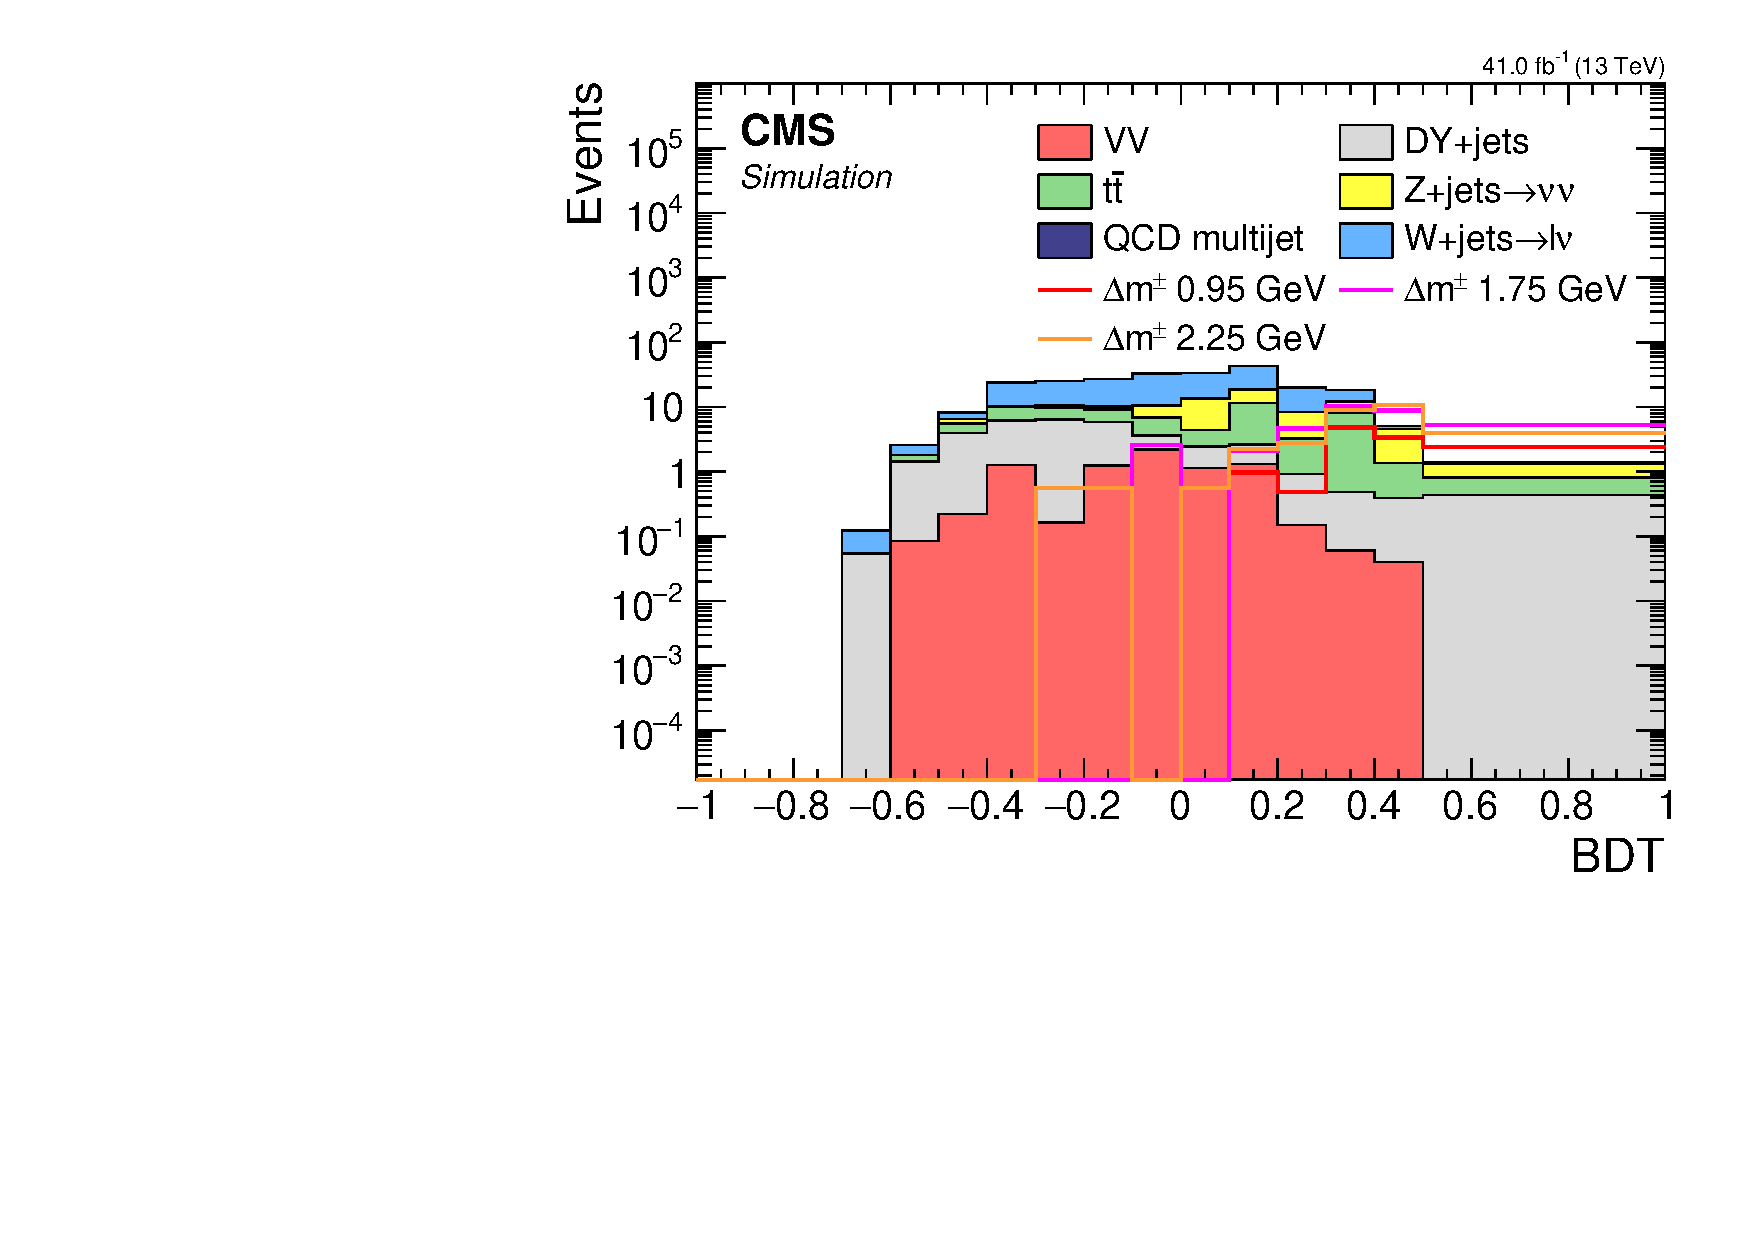
\includegraphics[width=0.48\linewidth]{plots/dilepton_muons_2017/none_custom_dilepBDTCorrJetNoMultIso10Dr0.6_log.pdf} \,
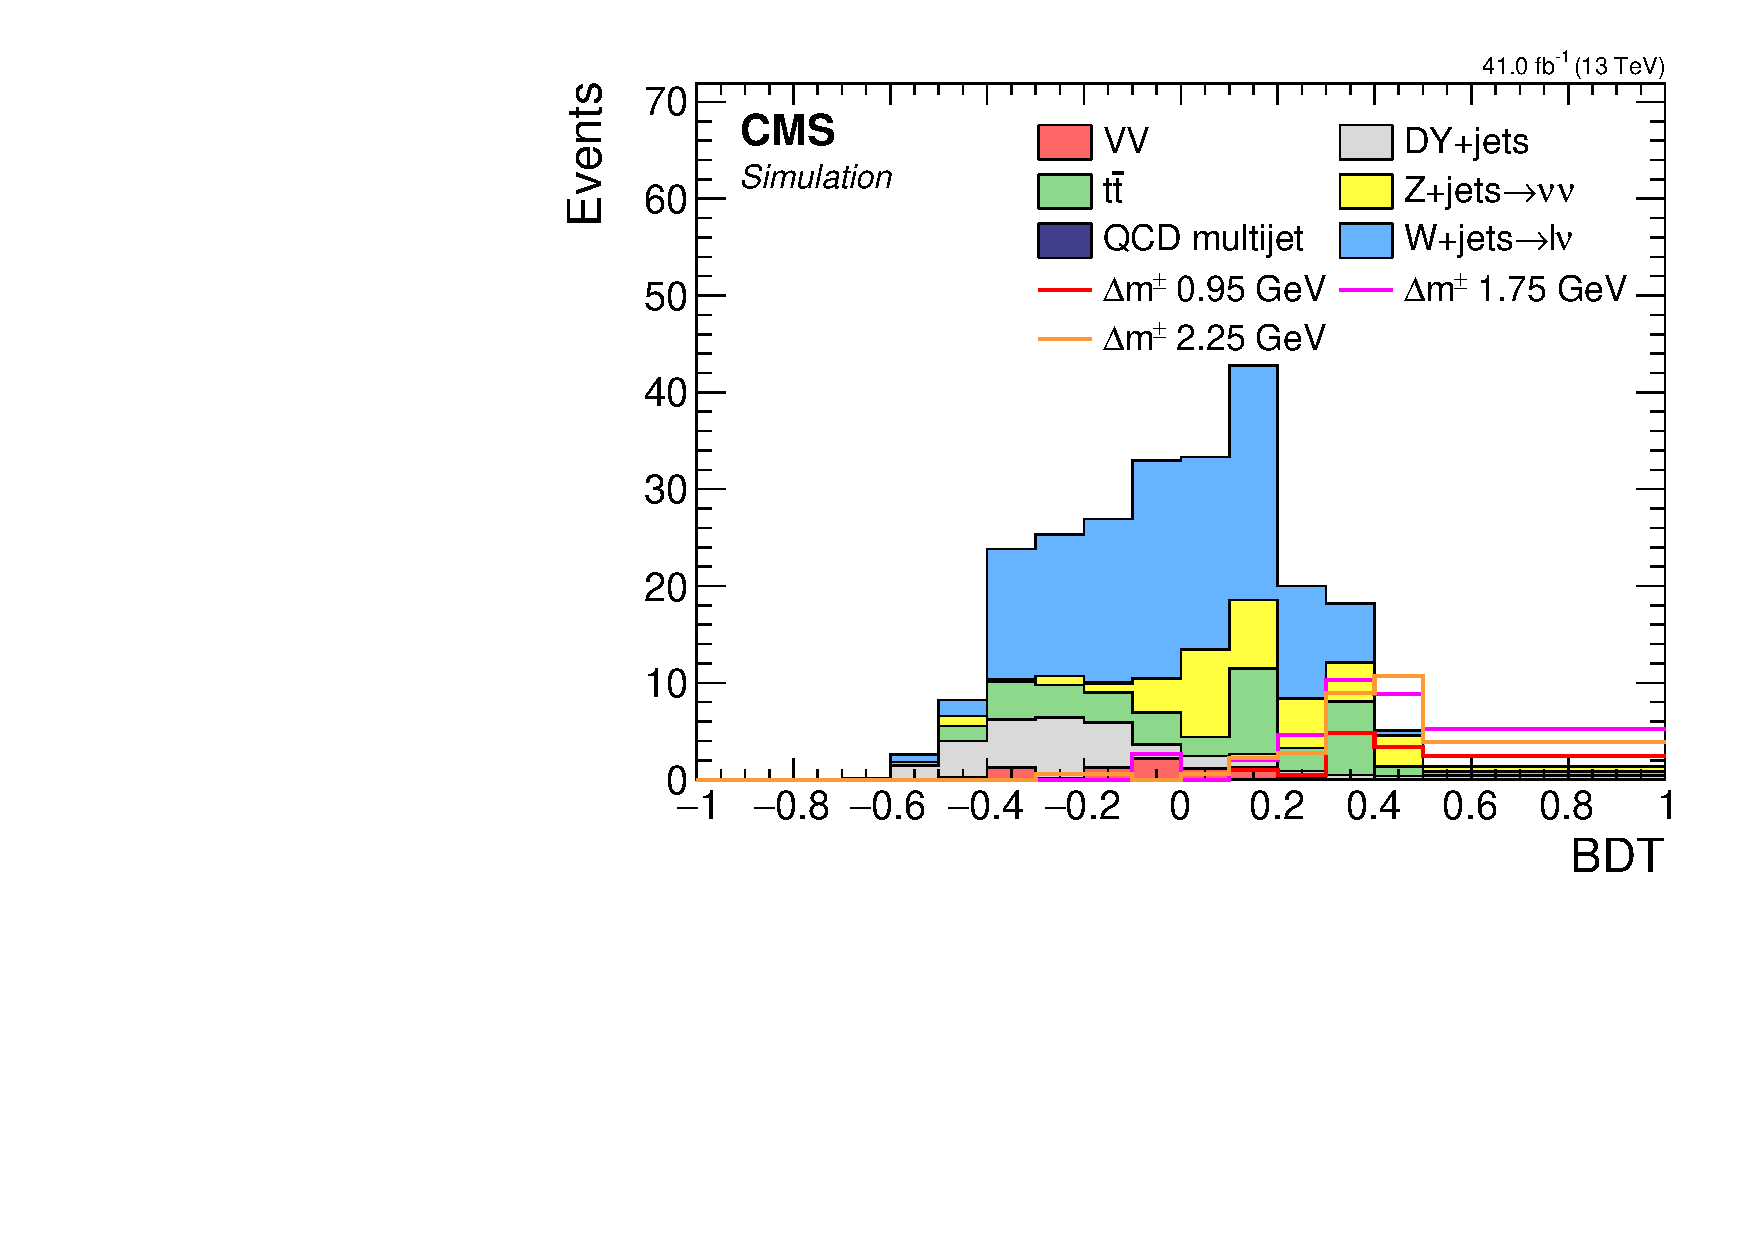
\includegraphics[width=0.48\linewidth]{plots/dilepton_muons_2017/none_custom_dilepBDTCorrJetNoMultIso10Dr0.6.pdf} \\


\caption[Dimuon simulation BDT output]{Dimuon 2017 simulation BDT score in log scale (left) and linear scale (right).}
\label{fig:dimuon-bdt-sim-output}
\end{figure}

\begin{figure}[!htb]
\centering
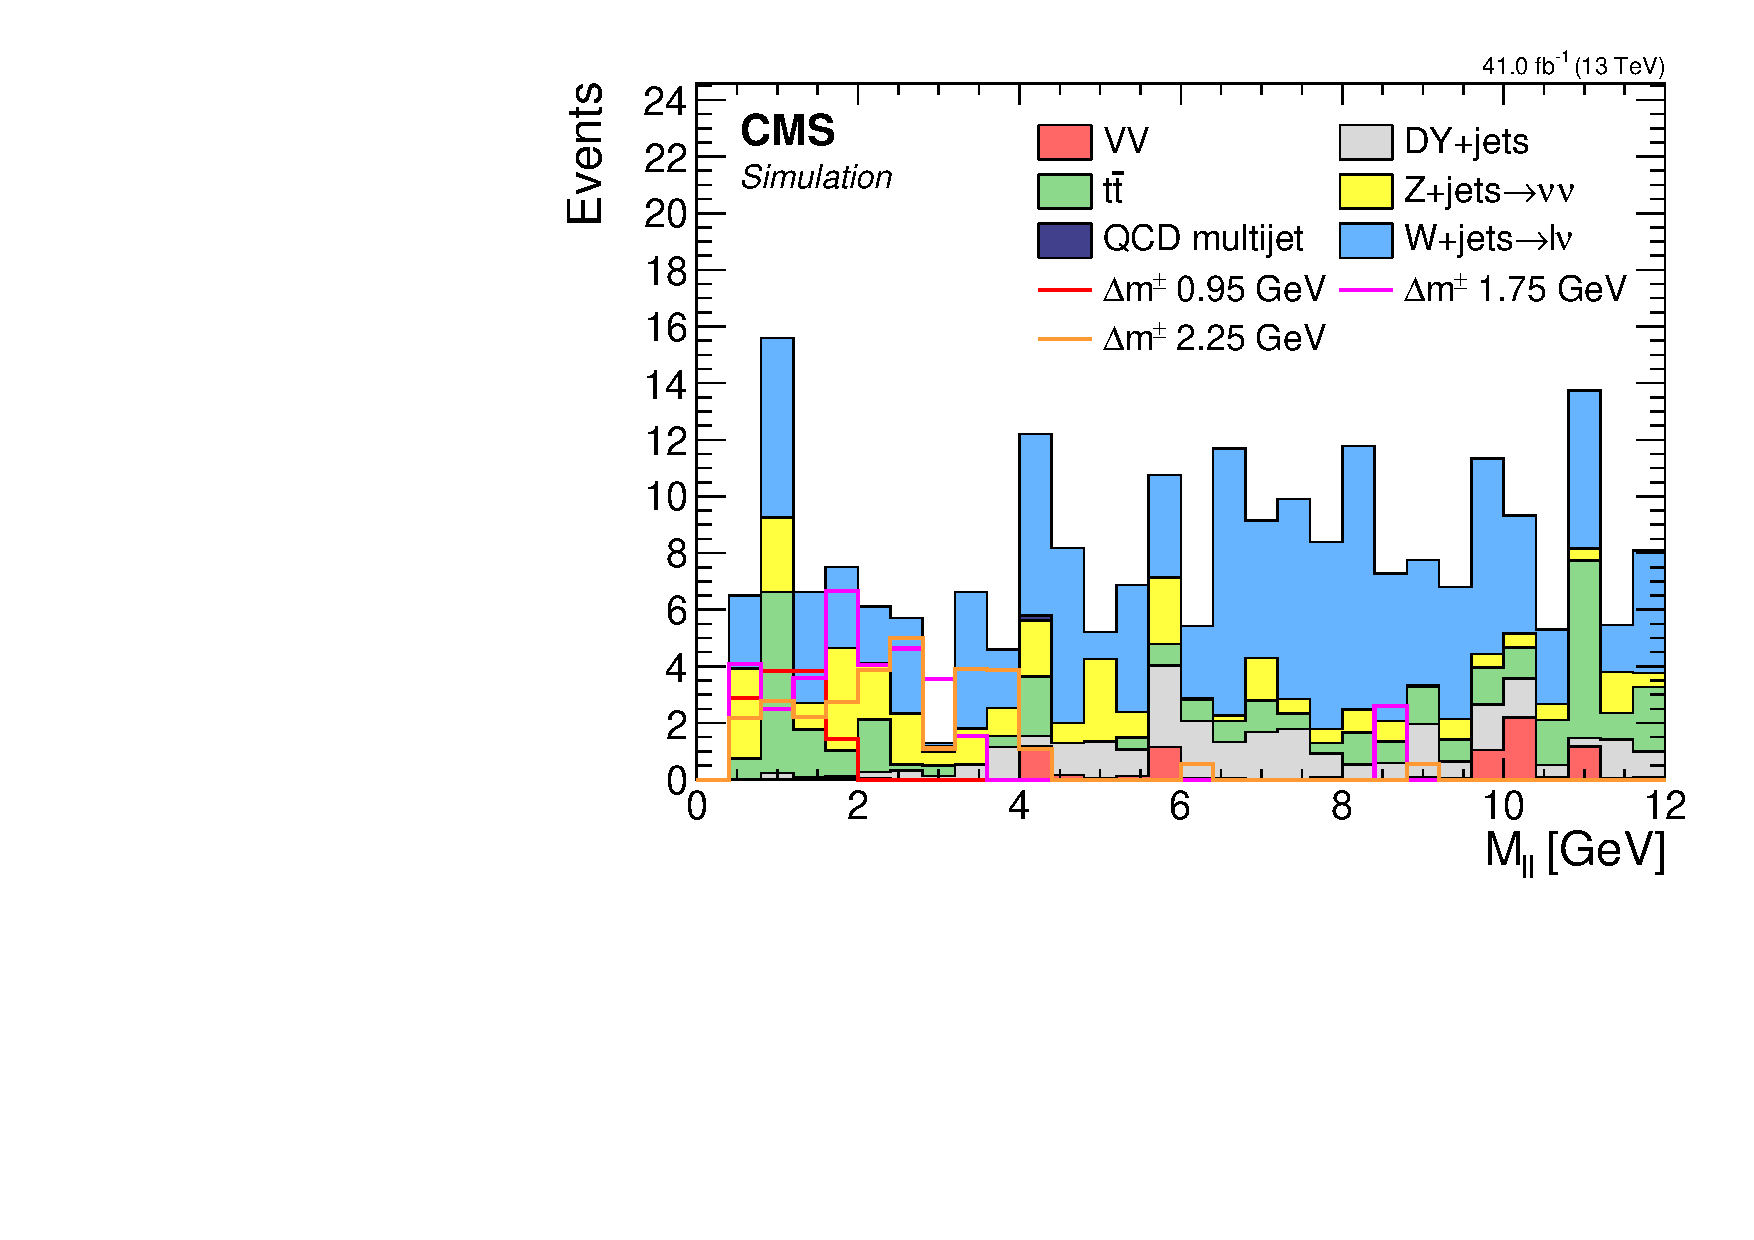
\includegraphics[width=0.48\linewidth]{plots/dilepton_muons_2017/none_invMassCorrJetNoMultIso10Dr0.6.pdf} \,
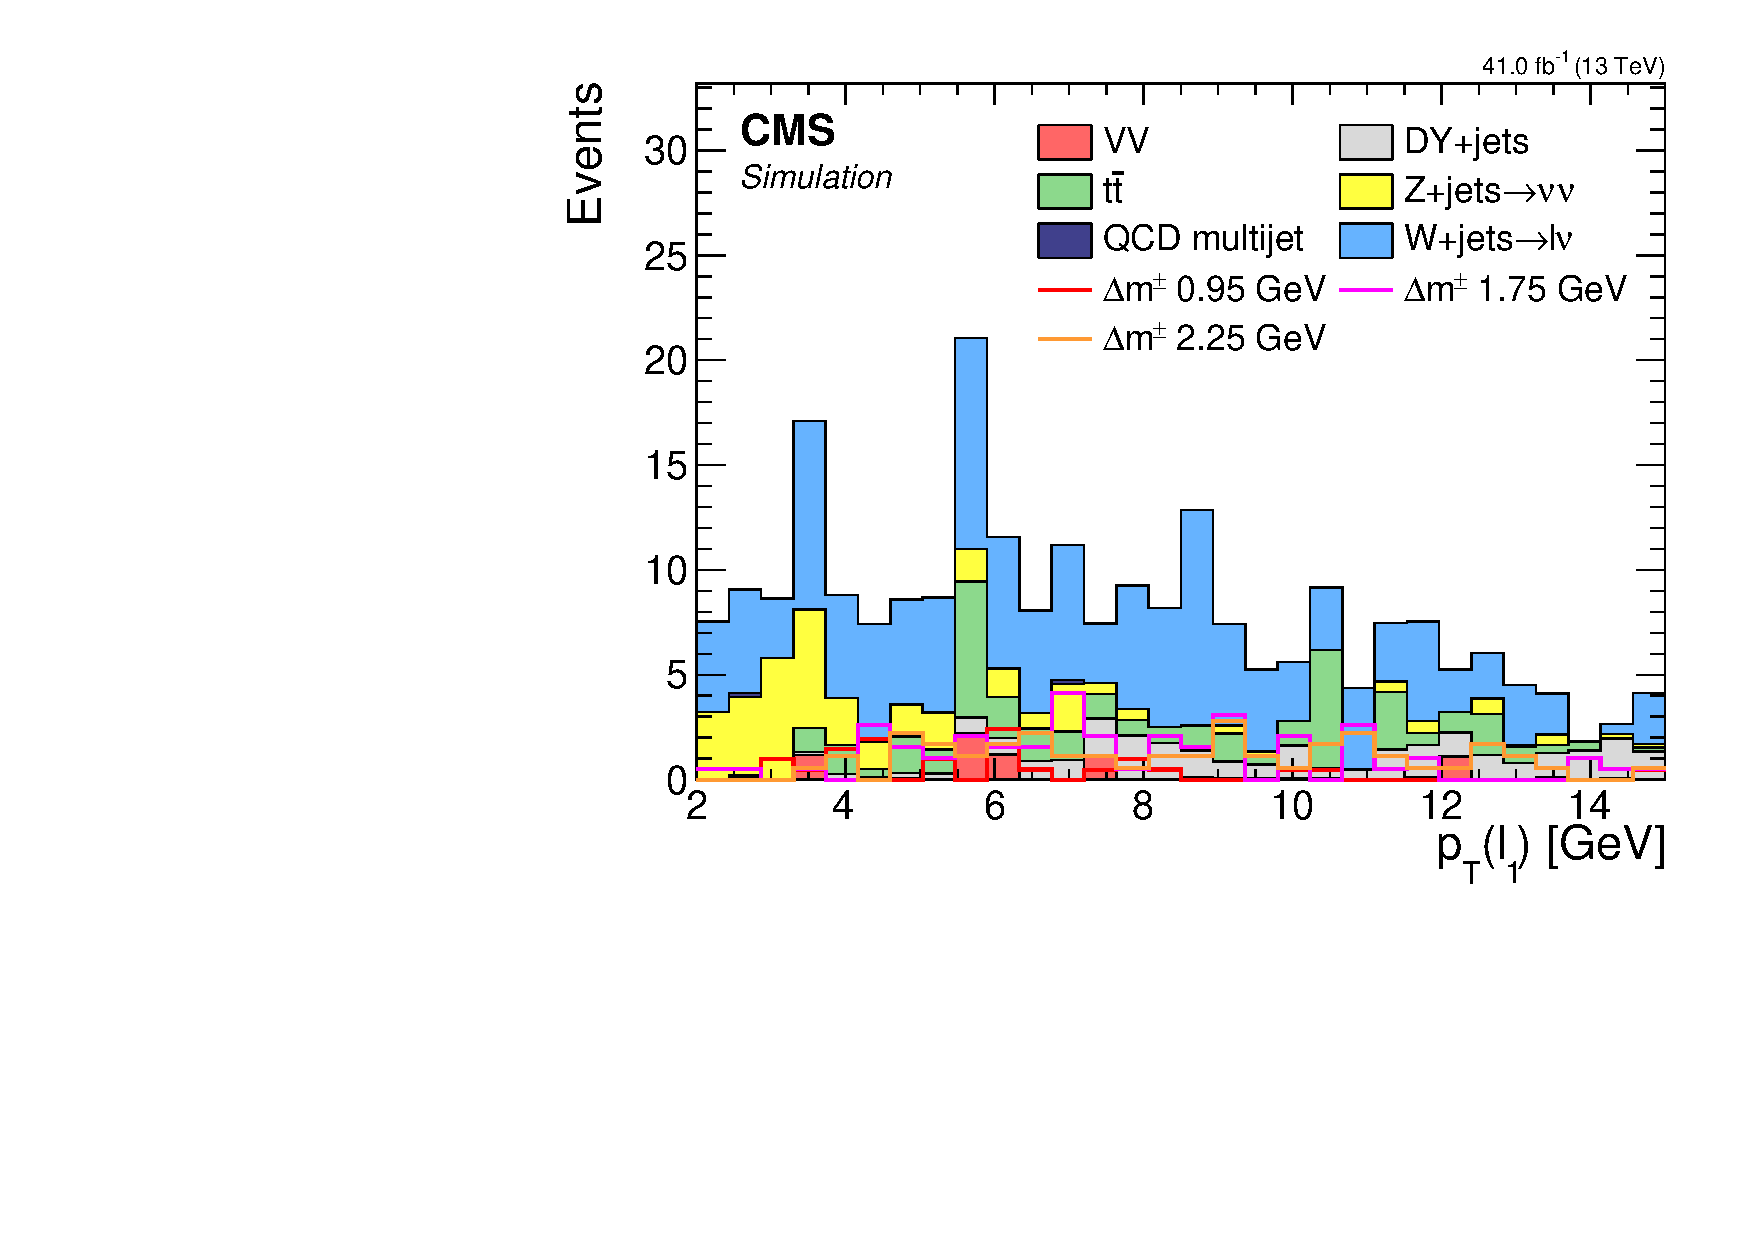
\includegraphics[width=0.48\linewidth]{plots/dilepton_muons_2017/none_leptonsCorrJetNoMultIso10Dr0.6[0].Pt(.pdf} \\

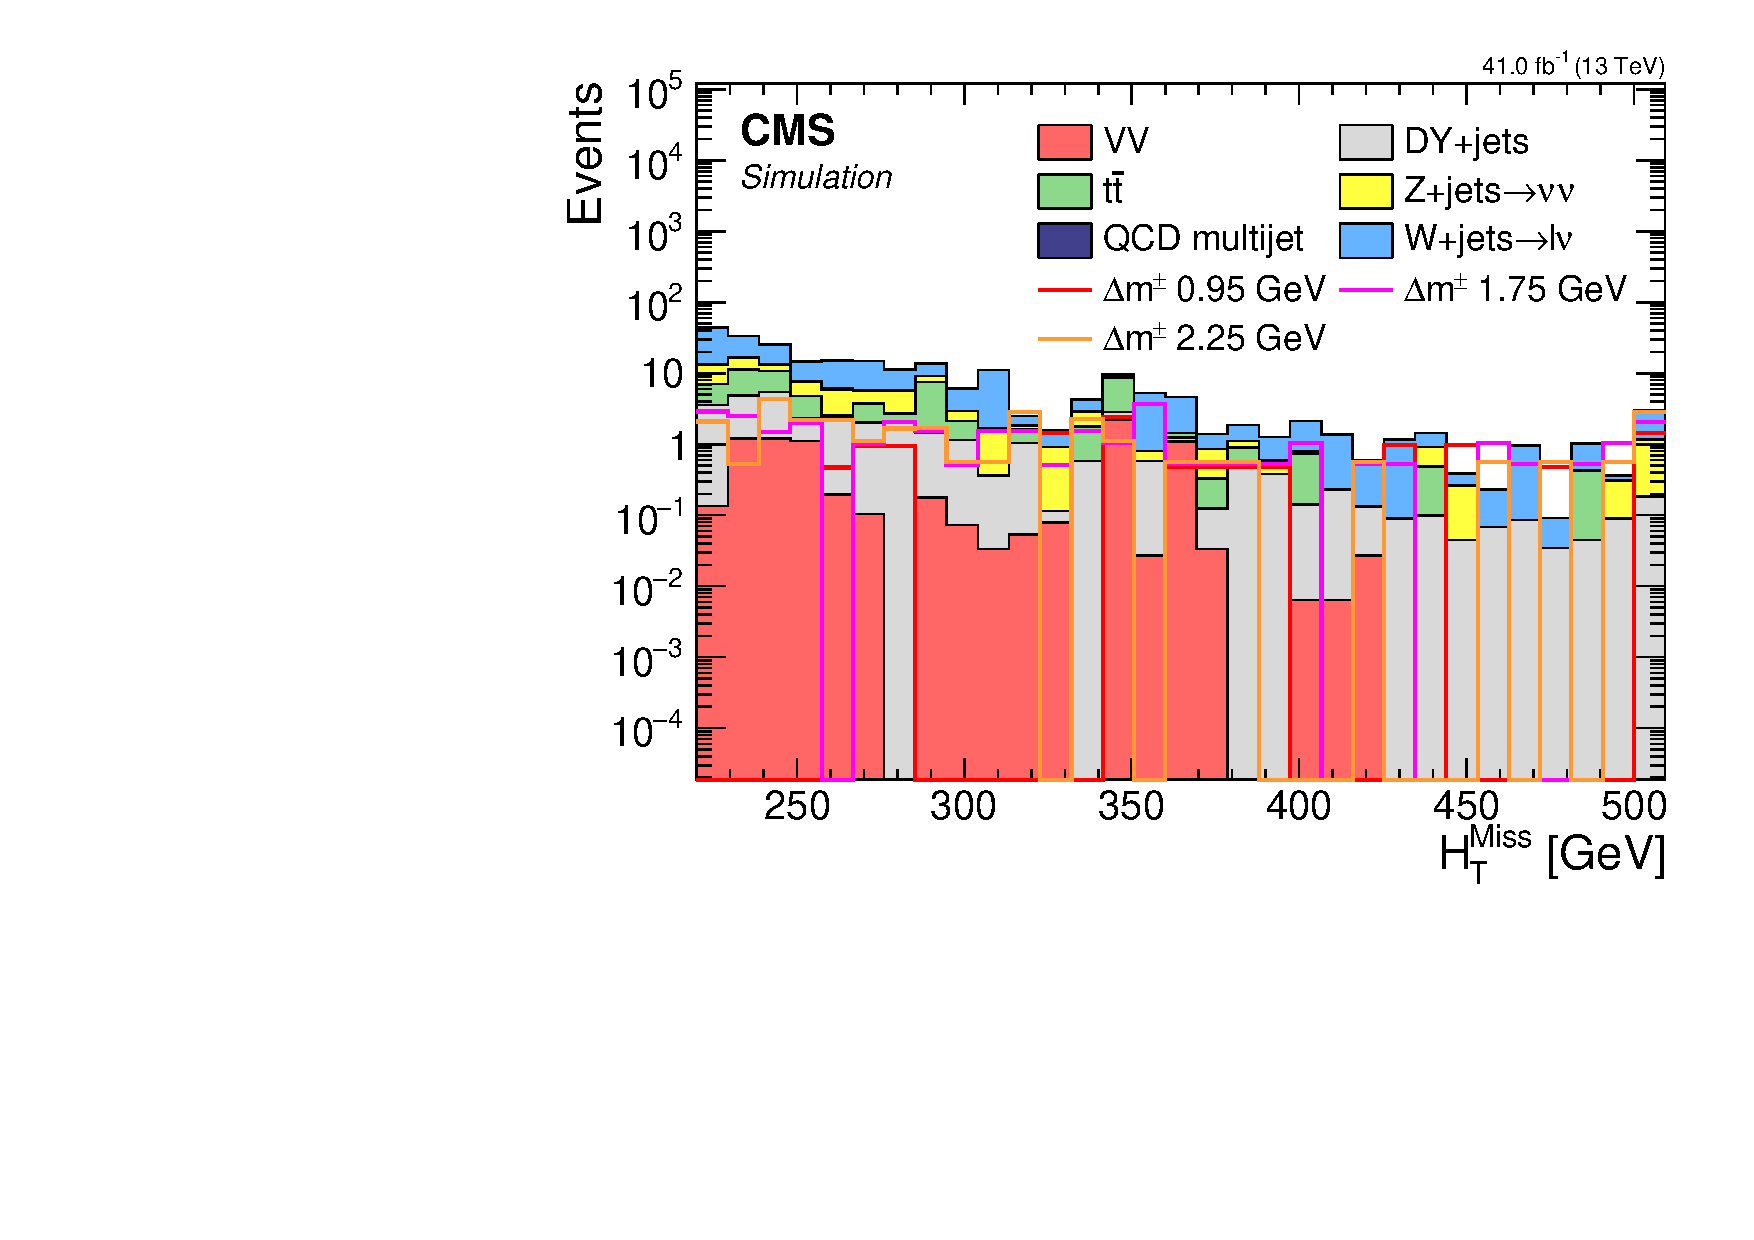
\includegraphics[width=0.48\linewidth]{plots/dilepton_muons_2017/none_MHT_log.pdf} \,
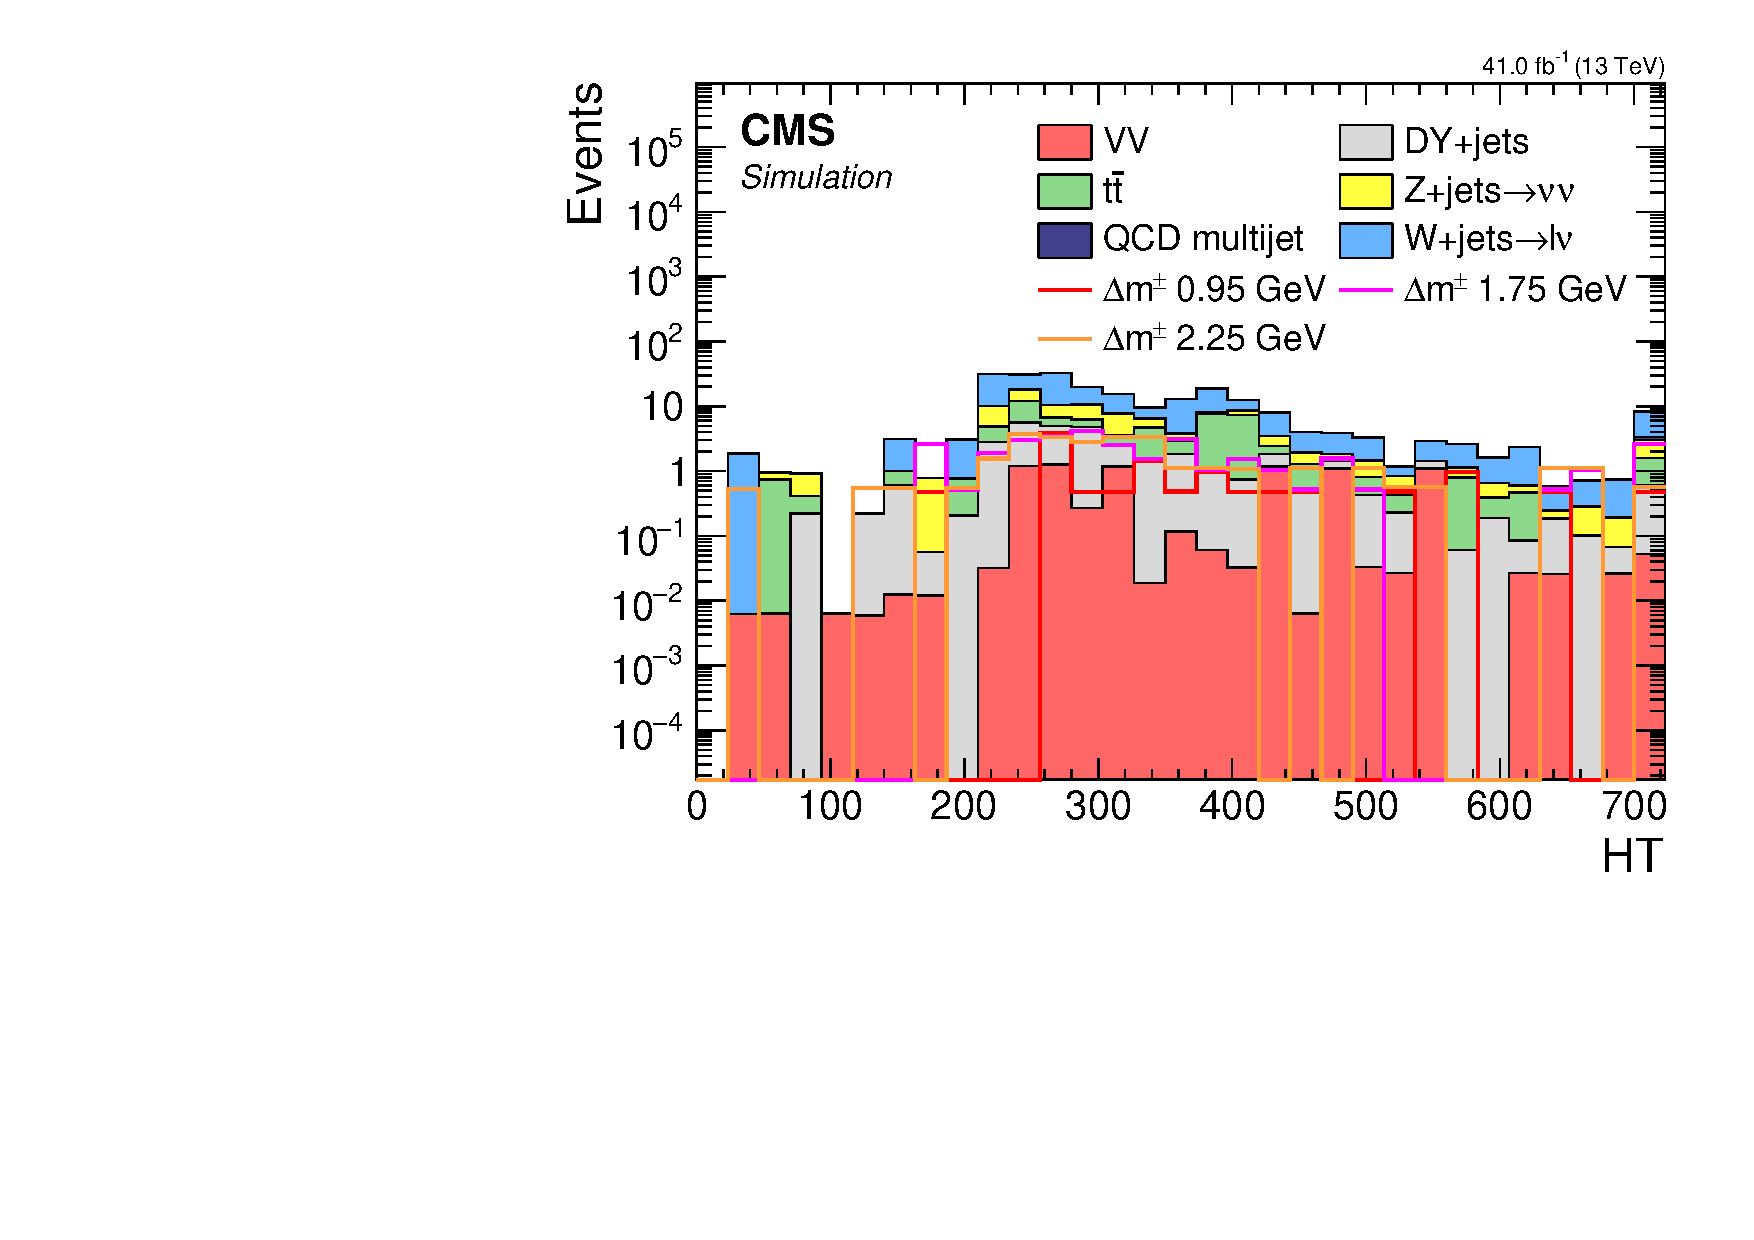
\includegraphics[width=0.48\linewidth]{plots/dilepton_muons_2017/none_HT_log.pdf} \\


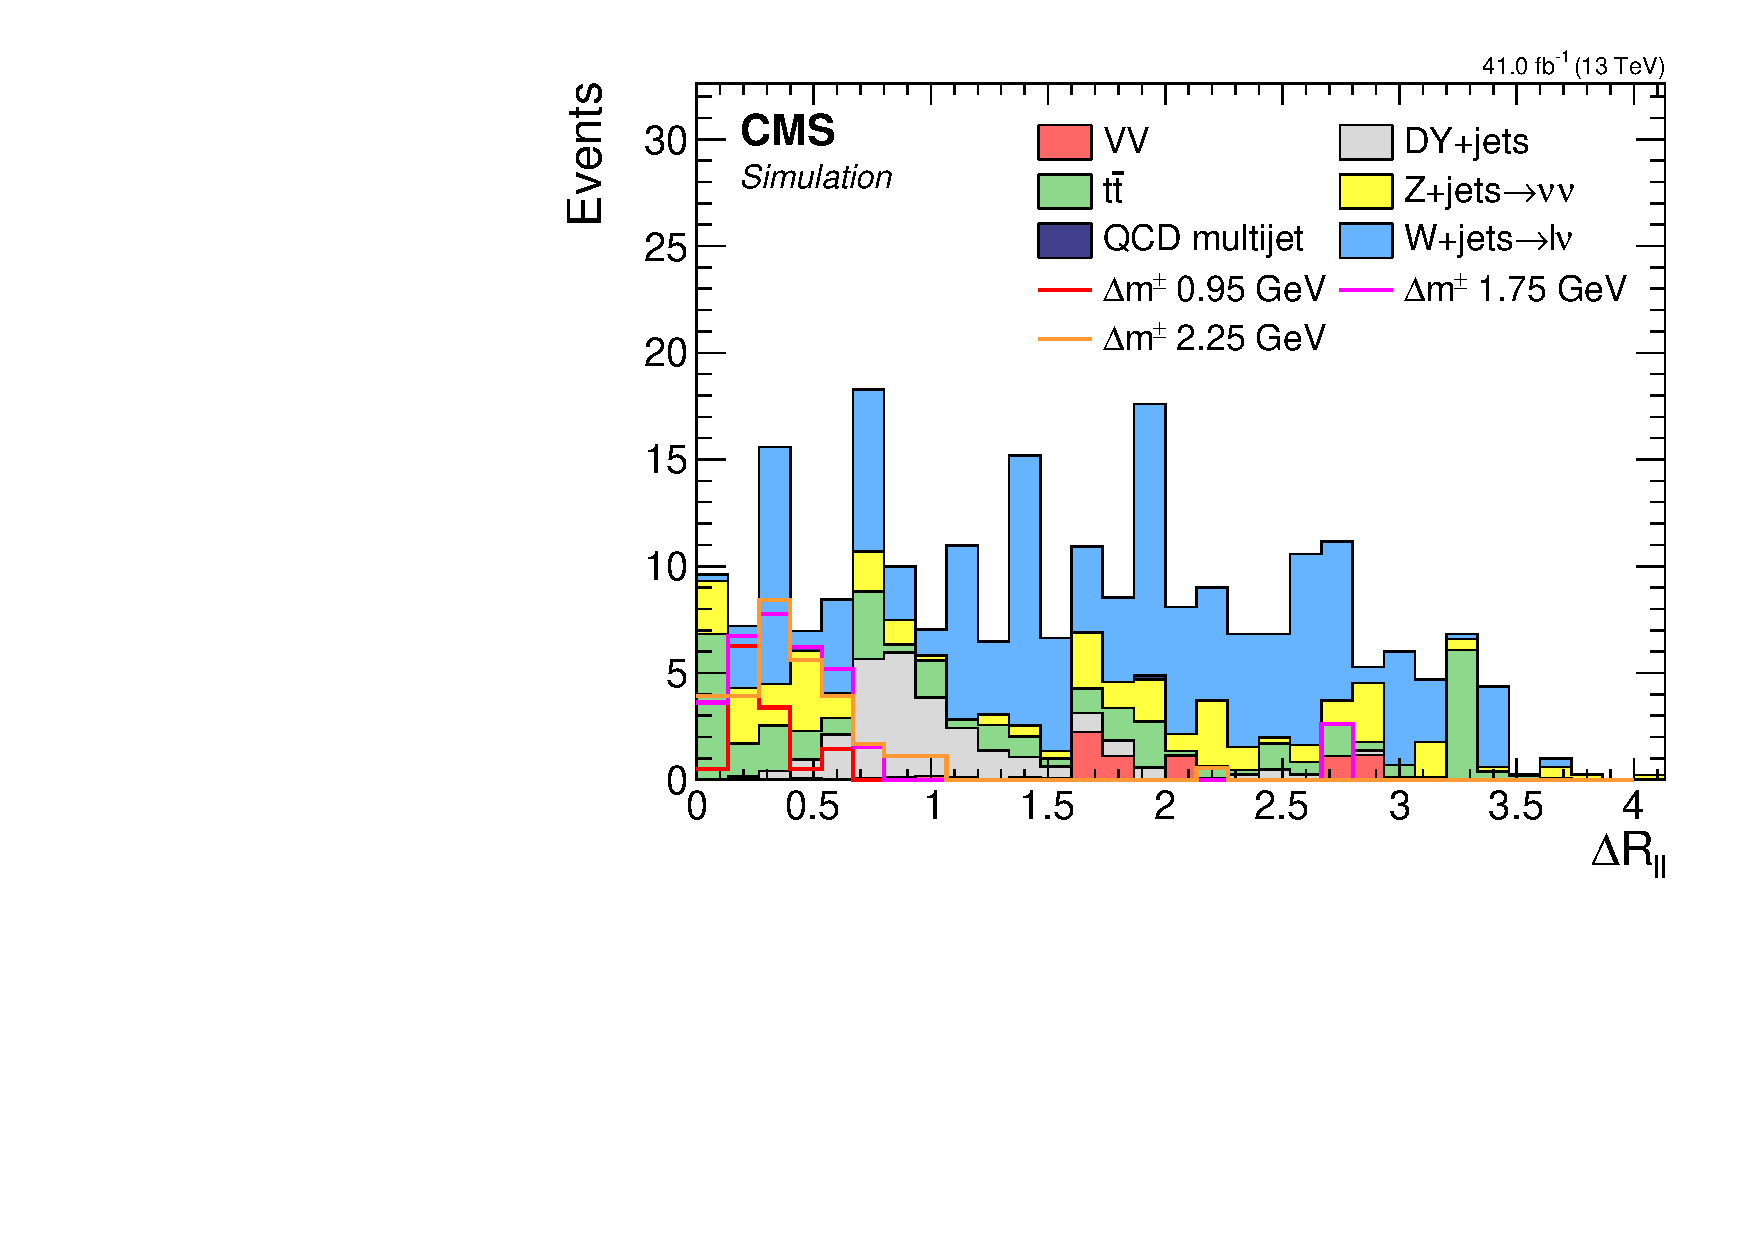
\includegraphics[width=0.48\linewidth]{plots/dilepton_muons_2017/none_deltaRCorrJetNoMultIso10Dr0.6.pdf} \,
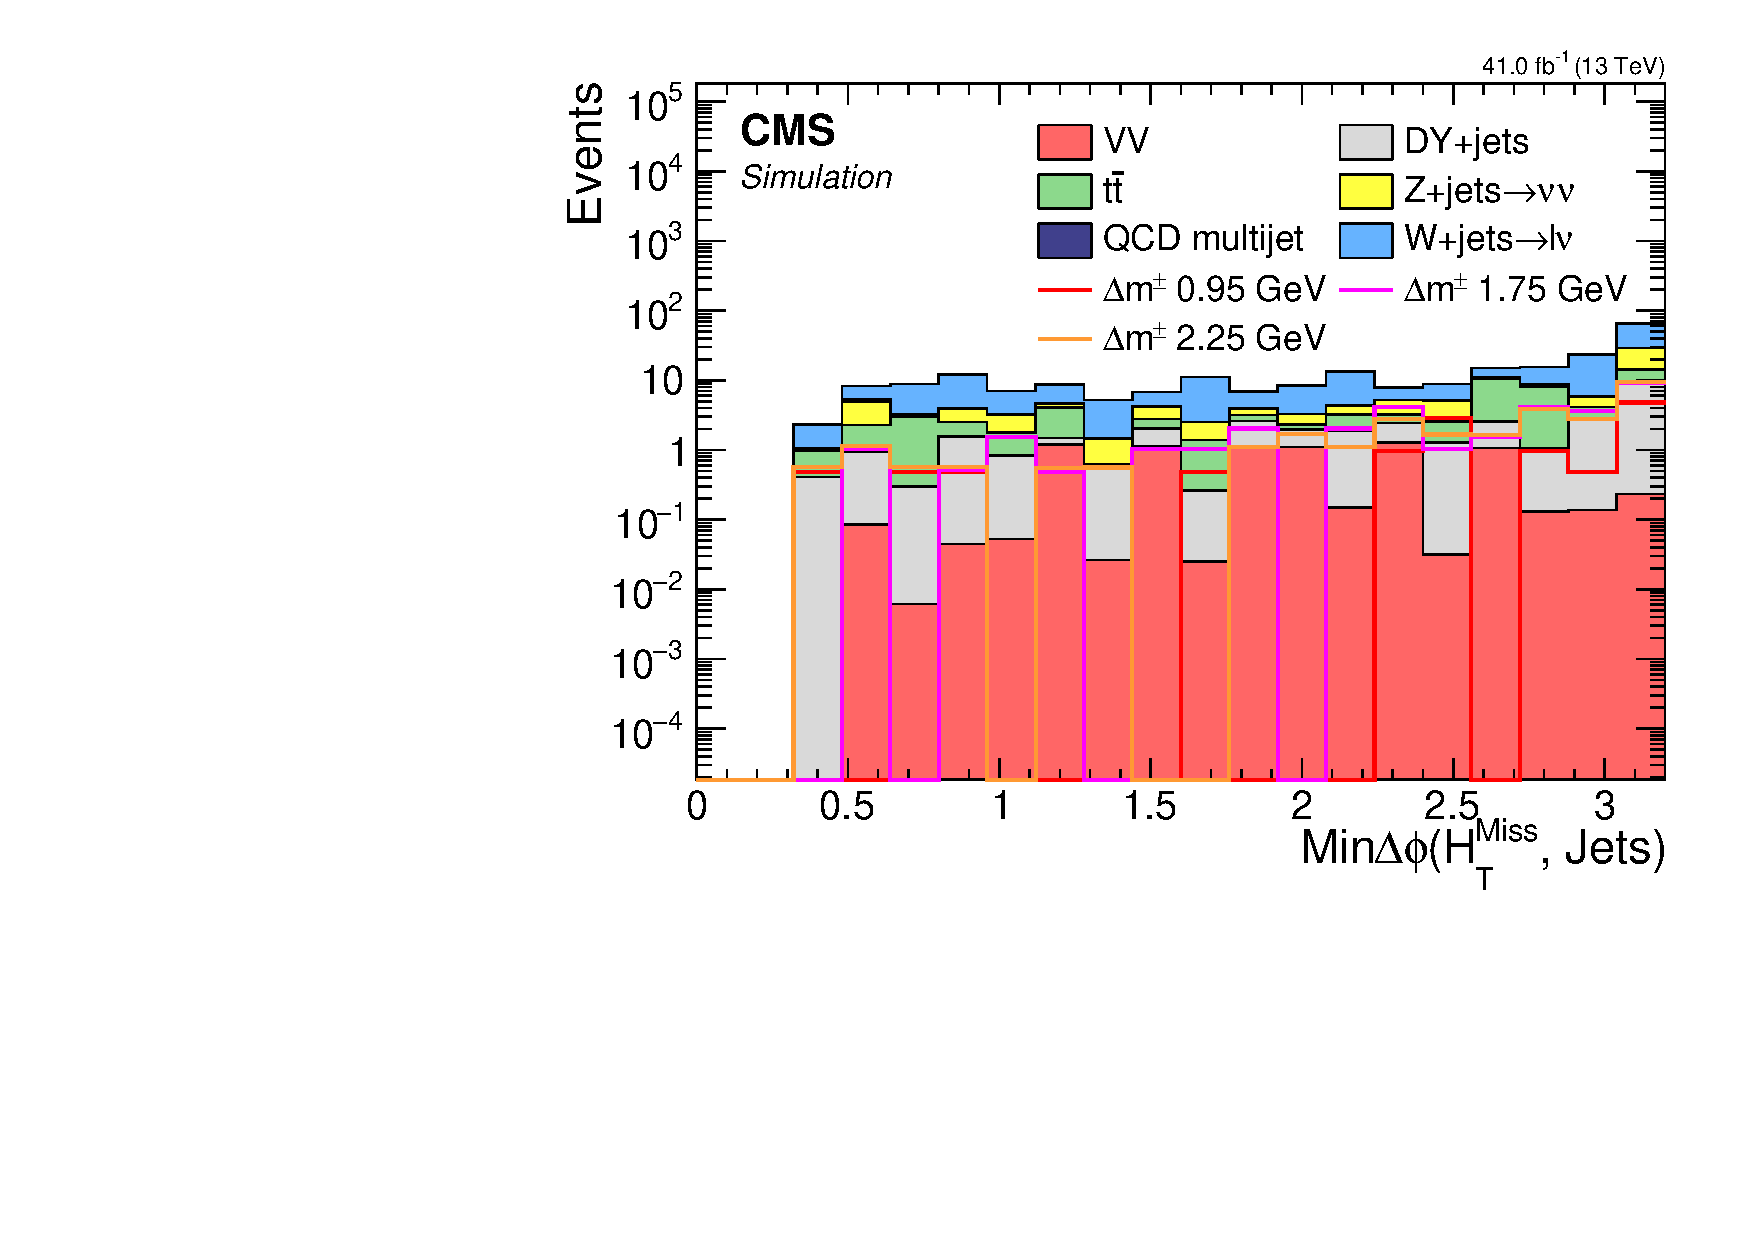
\includegraphics[width=0.48\linewidth]{plots/dilepton_muons_2017/none_MinDeltaPhiMhtJets_log.pdf} \\

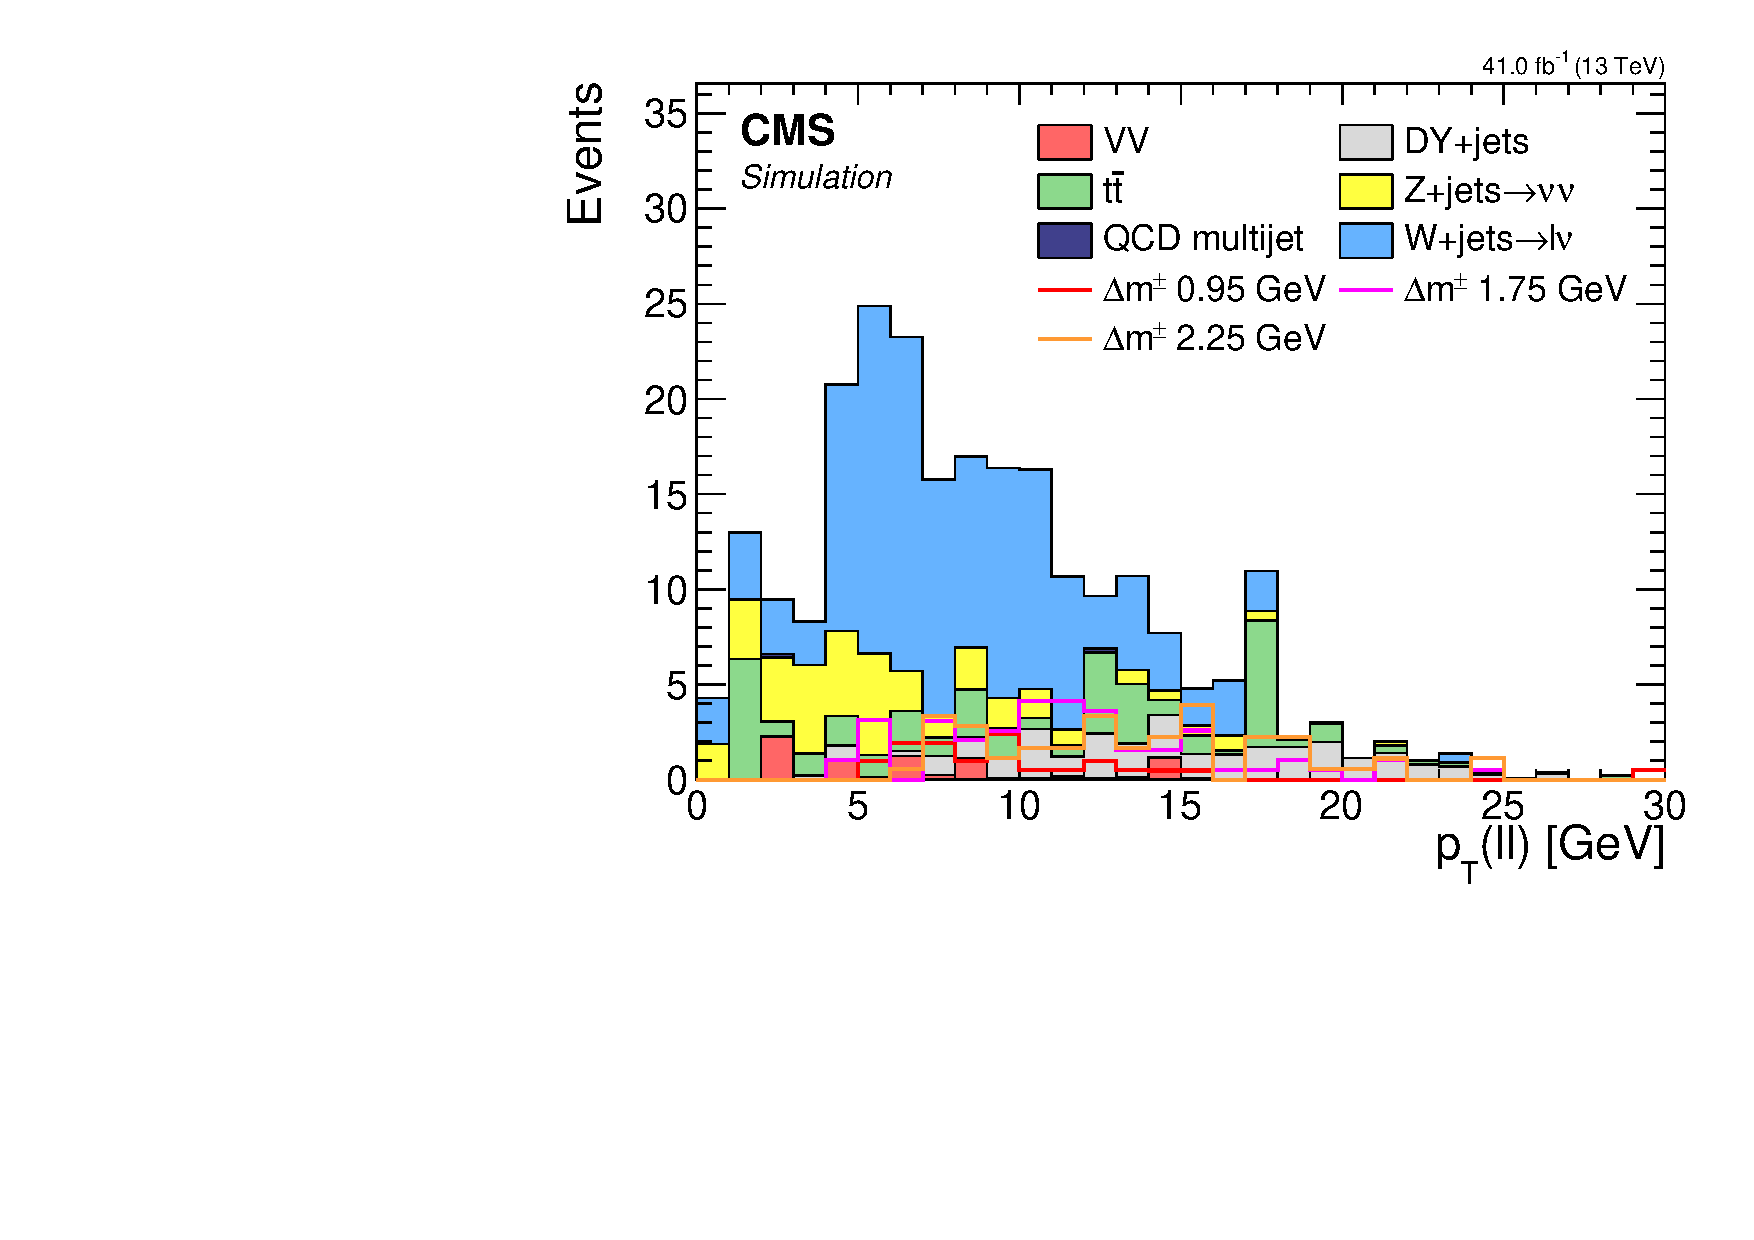
\includegraphics[width=0.48\linewidth]{plots/dilepton_muons_2017/none_dileptonPtCorrJetNoMultIso10Dr0.6.pdf} \,
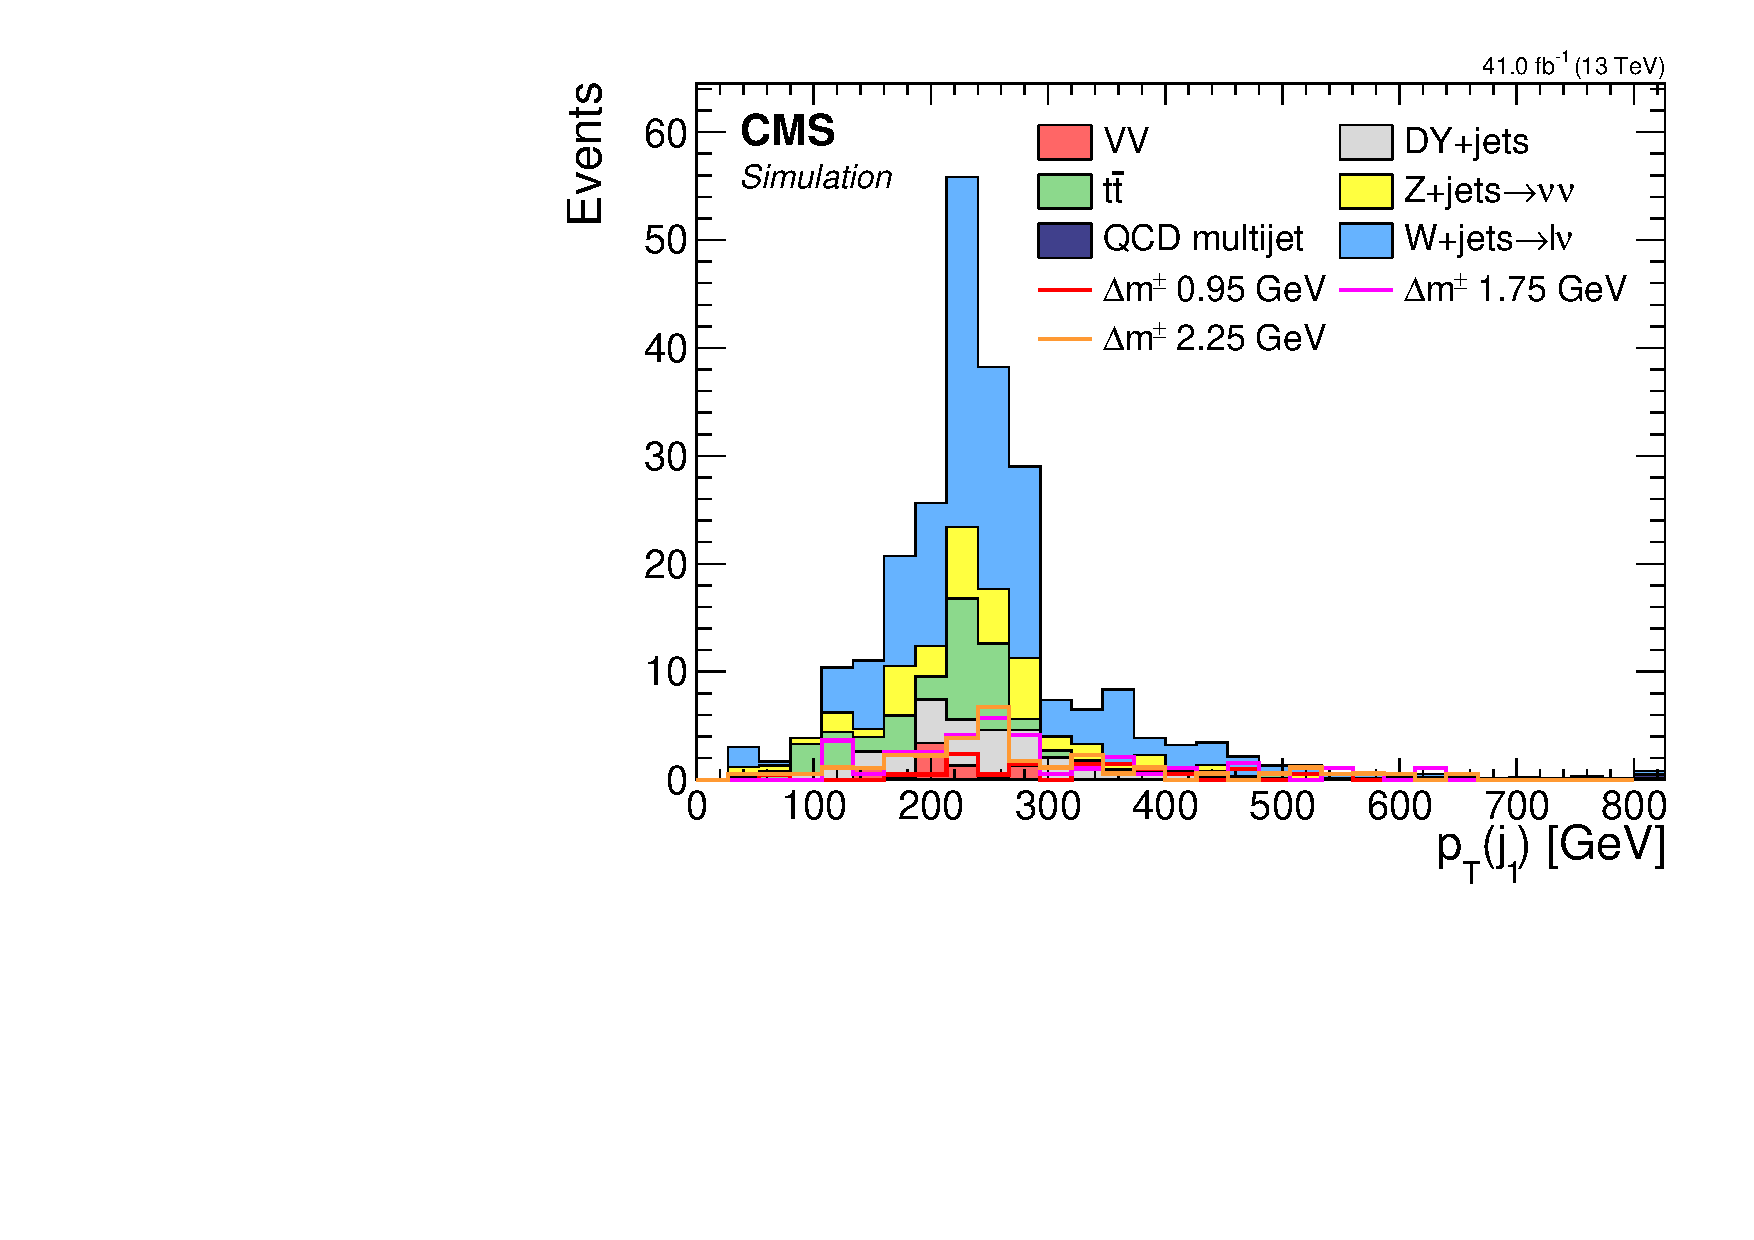
\includegraphics[width=0.48\linewidth]{plots/dilepton_muons_2017/none_LeadingJetPt.pdf} \\



\caption[Dimuon simulation BDT inputs]{Dimuon 2017 simulation BDT inputs for the top 10 ranked observables.}
\label{fig:dimuon-bdt-sim-inputs}
\end{figure}

\clearpage
\subsubsection{Exclusive track category}

As described before, there are four \glspl{bdt} in the exclusive track category, one for each of the two lepton flavors and each of two pixel tracker phases. The distribution of the muon+track category is shown in Figure~\ref{fig:exclusive-track-bdt-sim-output}. Figure~\ref{fig:exclusive-track-muon-bdt-sim-inputs} shows the top eight input observables to the \gls{bdt}, ranked by importance for the classifier. It is weighted to 2017 luminosity and uses 2017 simulated data. A few signal points are to indicate the signal-like regions of phase space. 

\begin{figure}[!htb]
\centering
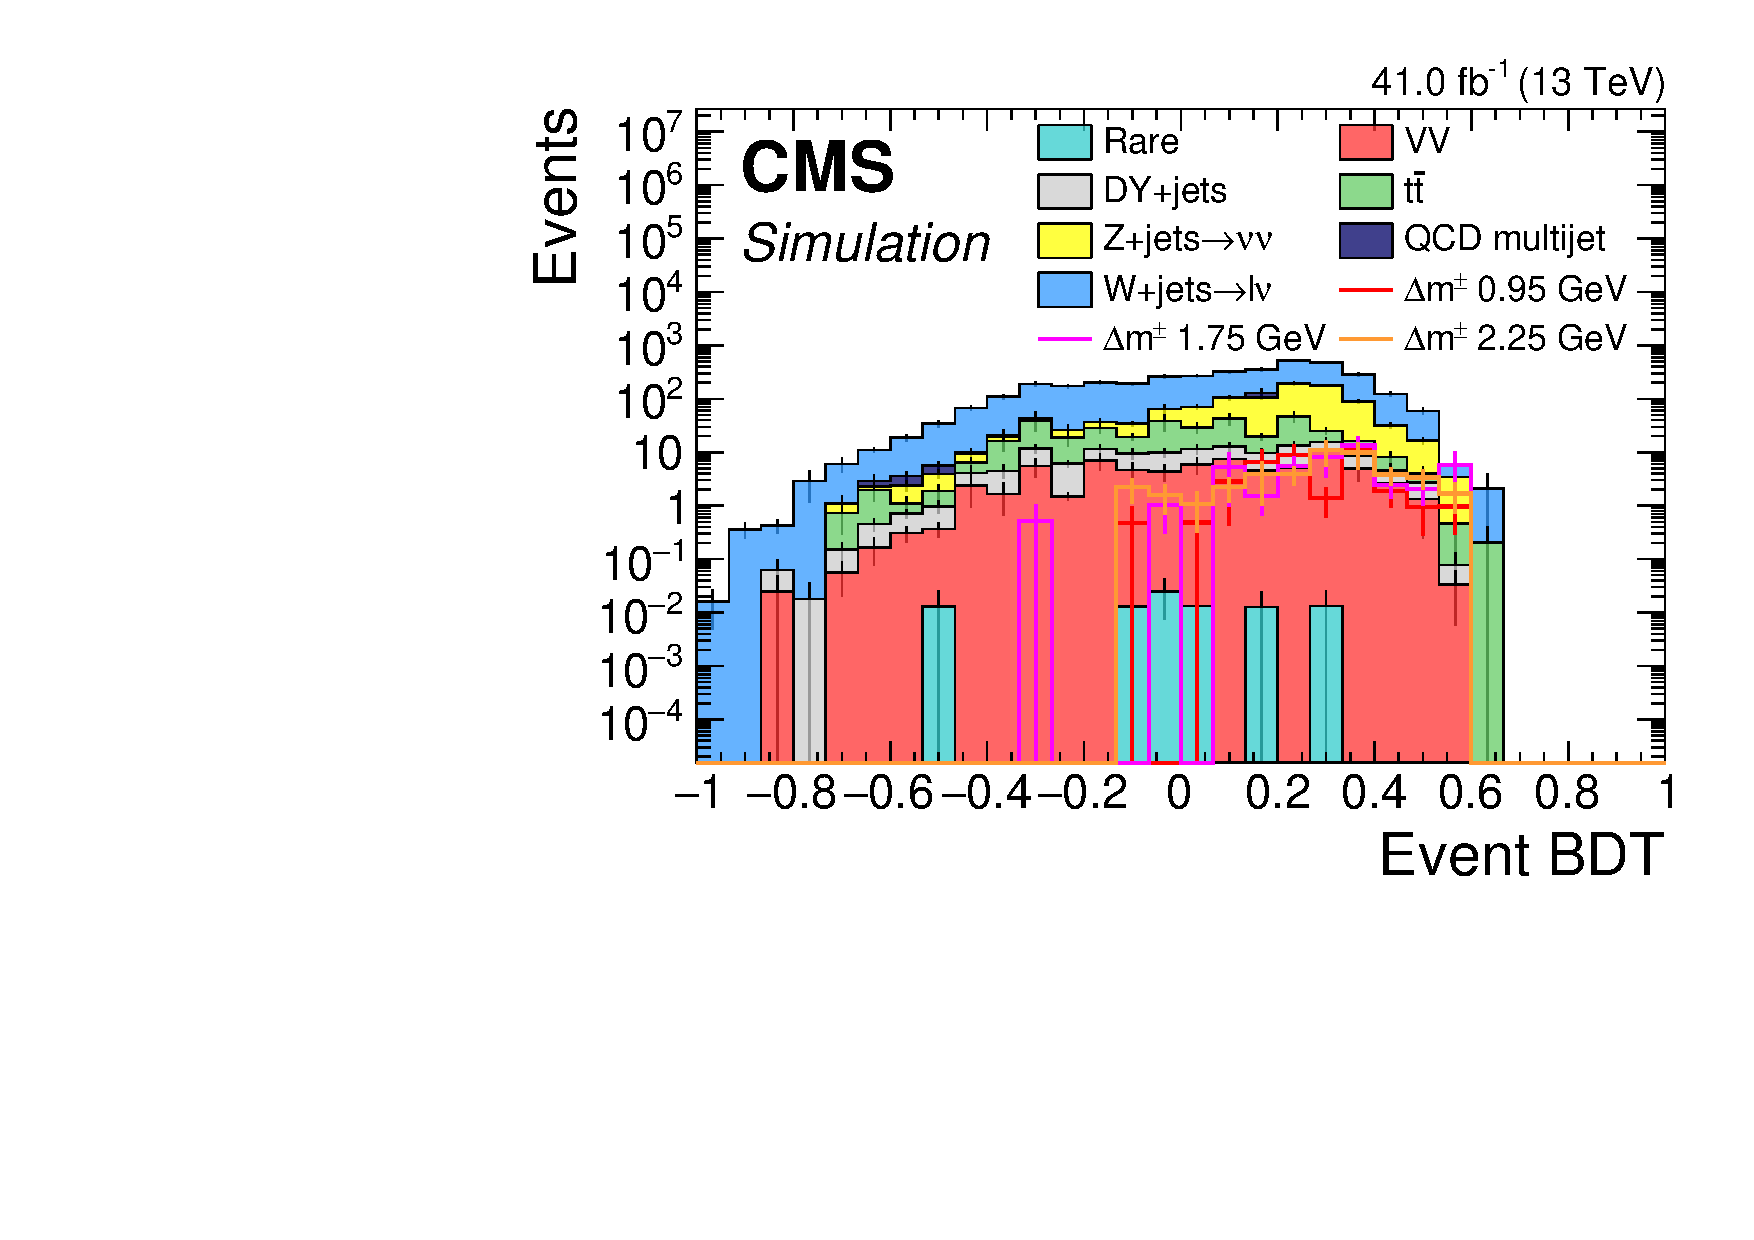
\includegraphics[width=0.48\linewidth]{plots/track_muon_bg_signal/none_exTrack_dilepBDTCorrJetNoMultIso10Dr0.6_log.pdf} \,
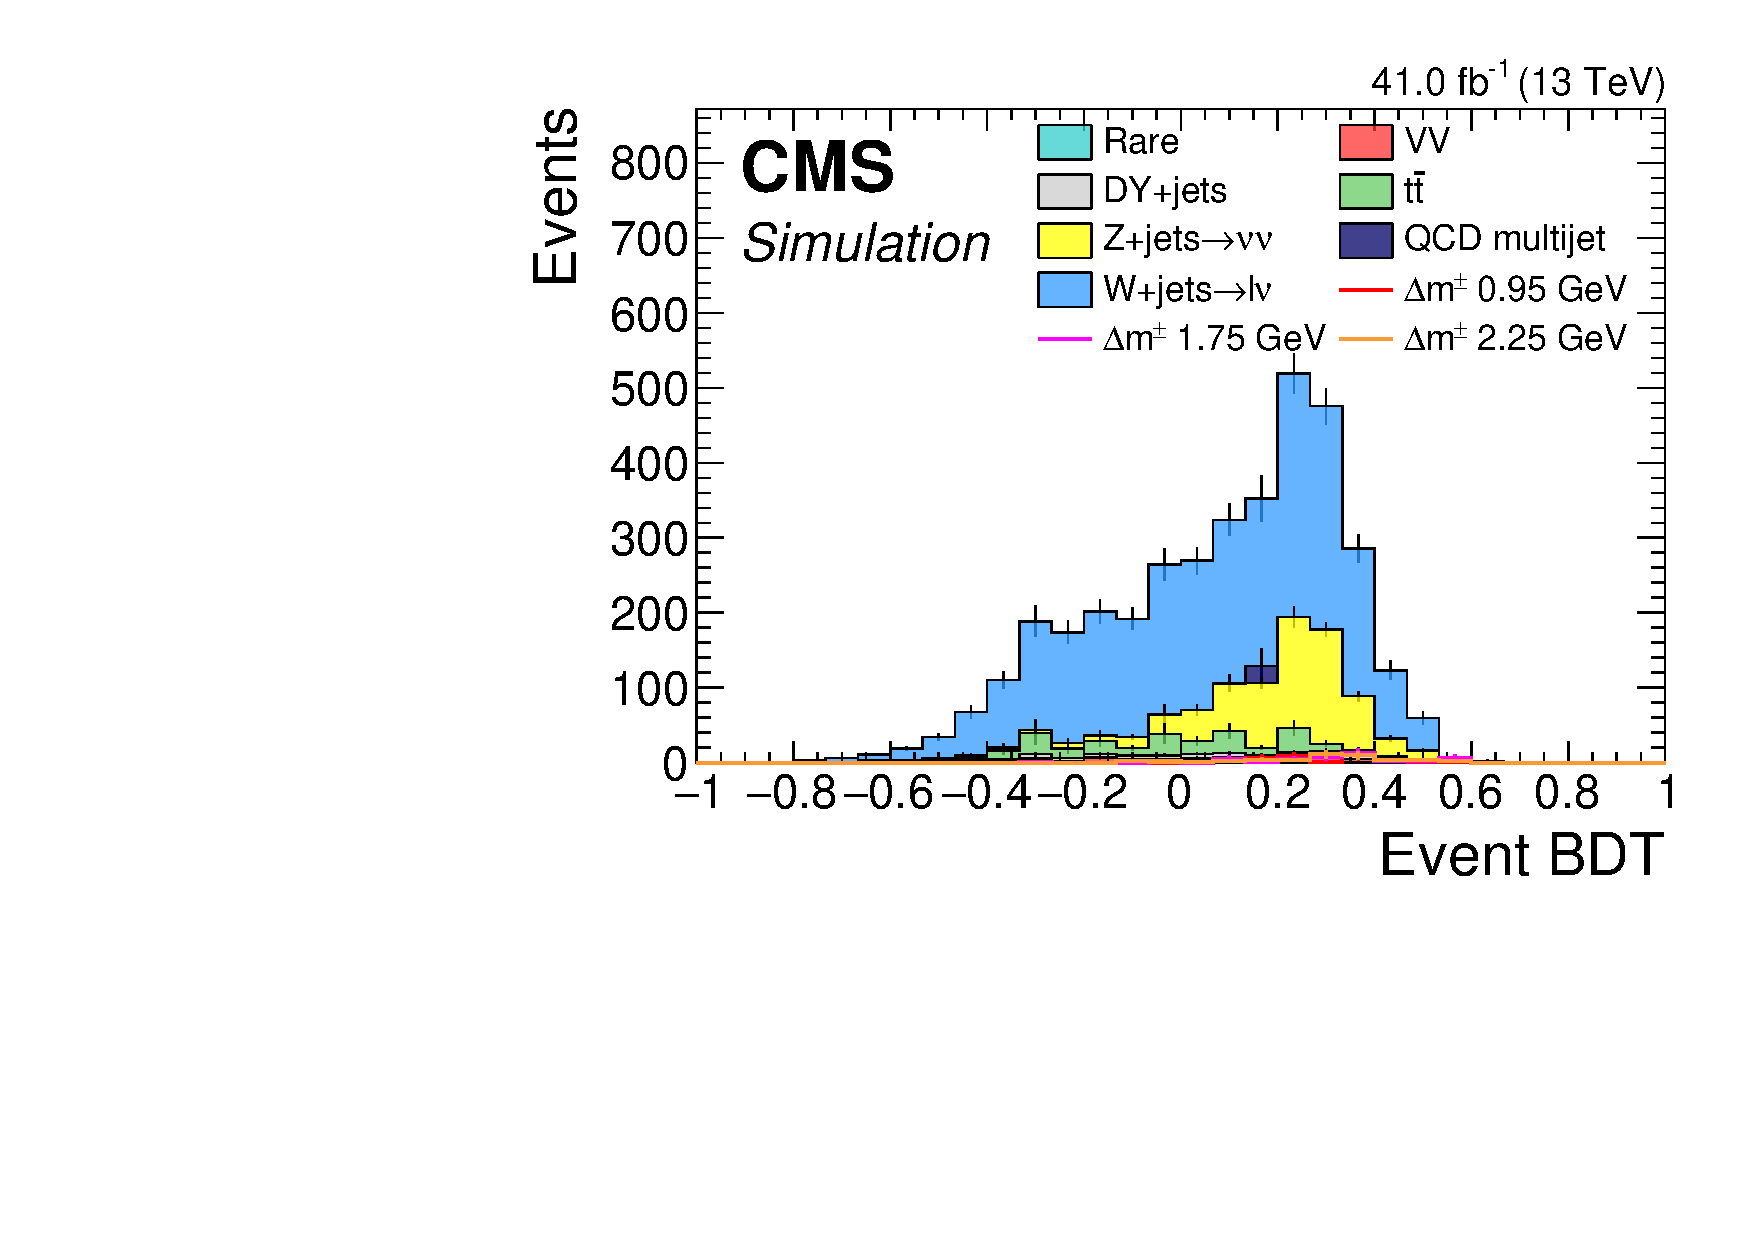
\includegraphics[width=0.48\linewidth]{plots/track_muon_bg_signal/none_exTrack_dilepBDTCorrJetNoMultIso10Dr0.6.pdf} \\

\caption[Exclusive track plus muon 2017 simulation BDT output]{track+muon category 2017 simulation BDT output in log scale (left) and linear scale (right).}
\label{fig:exclusive-track-bdt-sim-output}
\end{figure}

\begin{figure}[!htb]
\centering
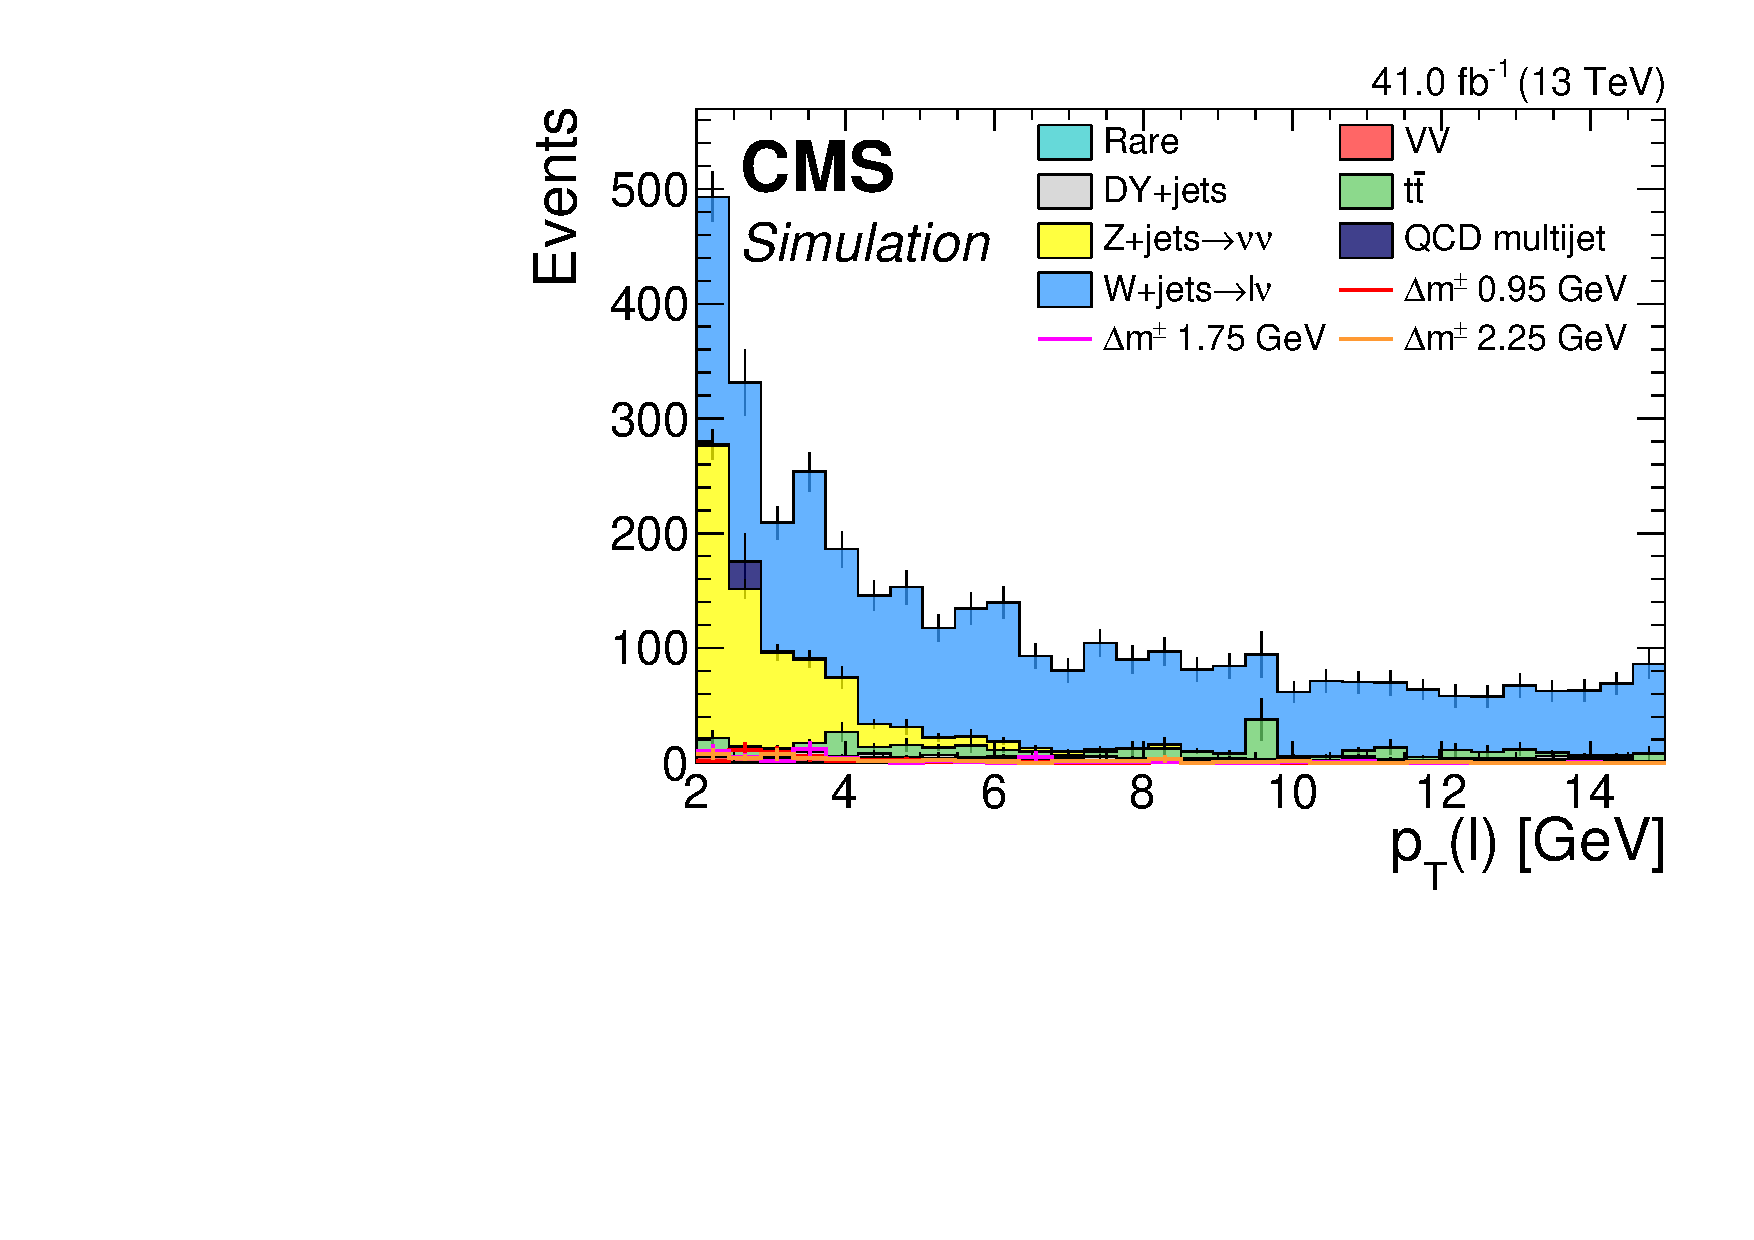
\includegraphics[width=0.48\linewidth]{plots/track_muon_bg_signal/none_leptonCorrJetNoMultIso10Dr0.6.Pt().pdf} \,
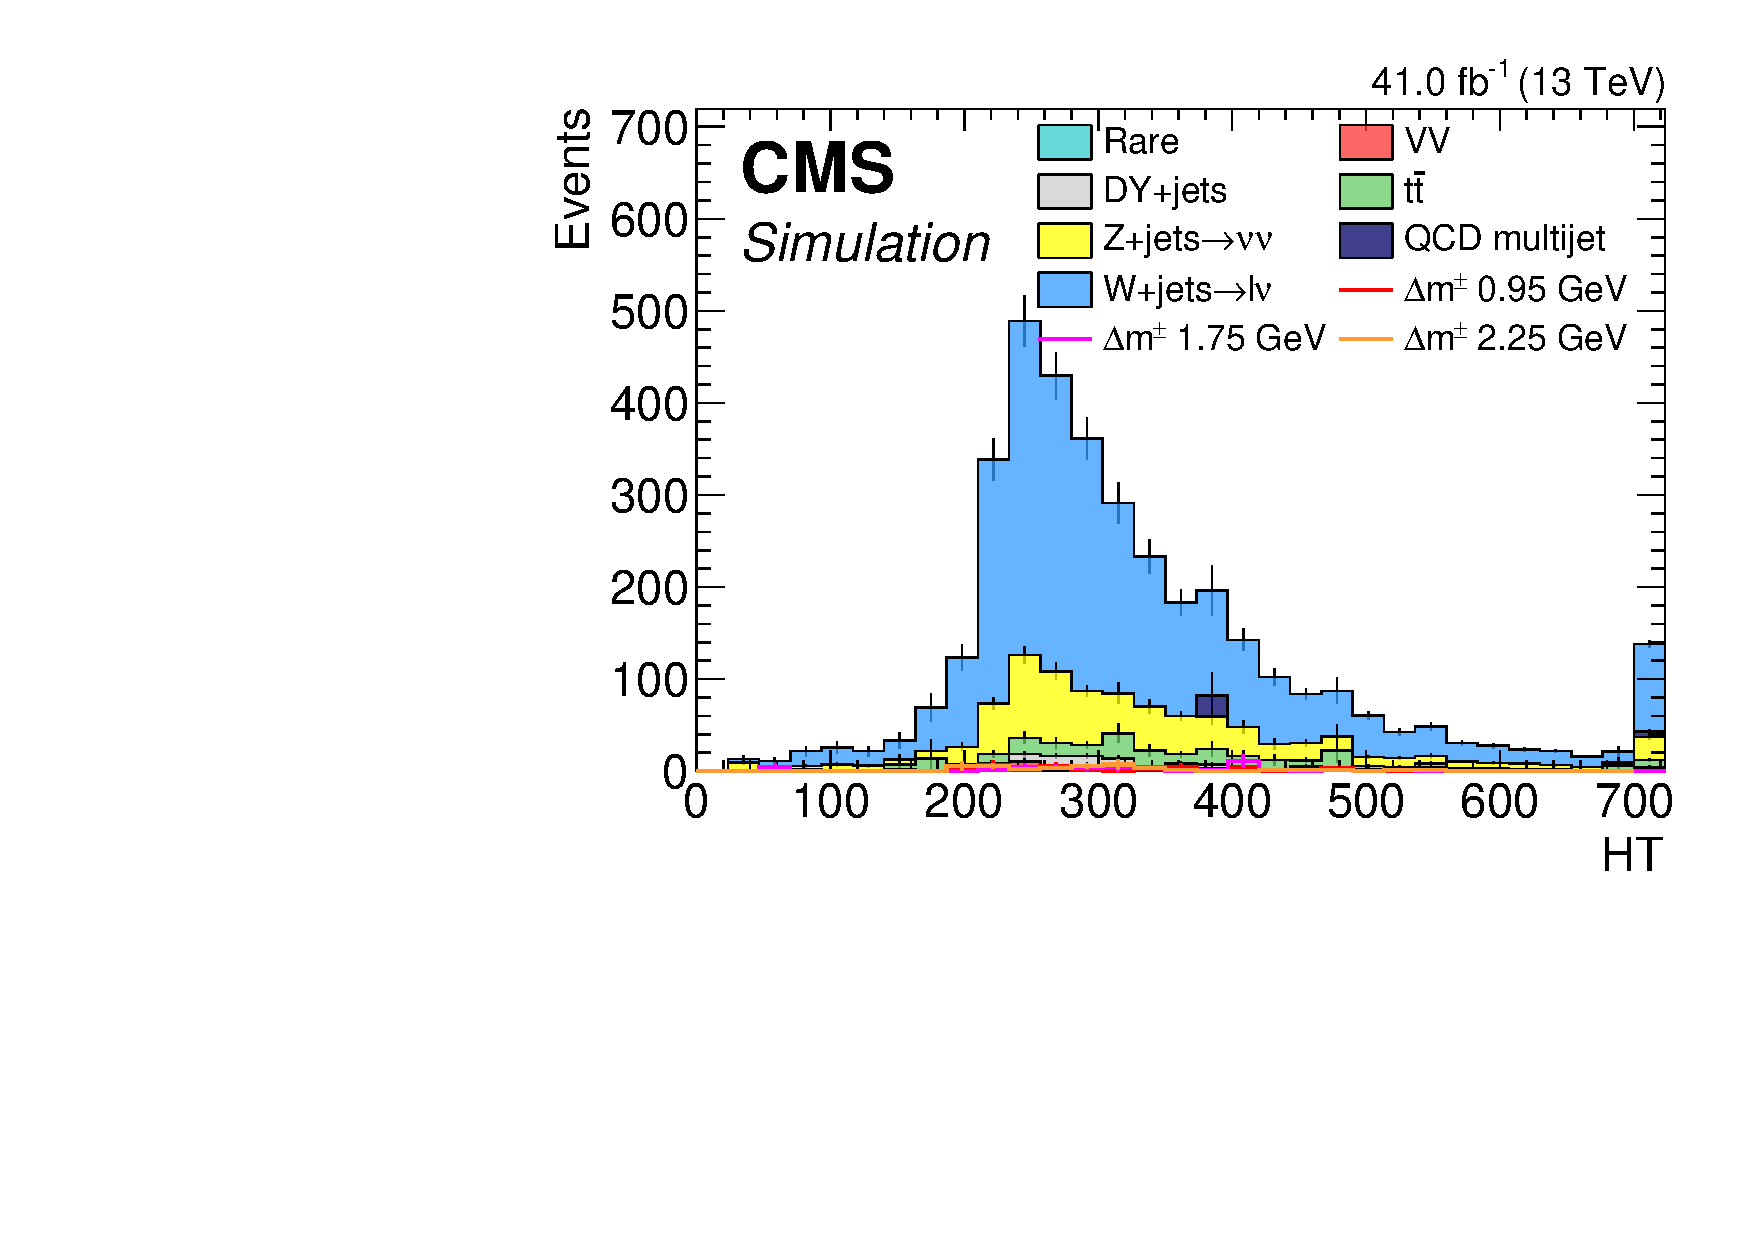
\includegraphics[width=0.48\linewidth]{plots/track_muon_bg_signal/none_HT.pdf} \\
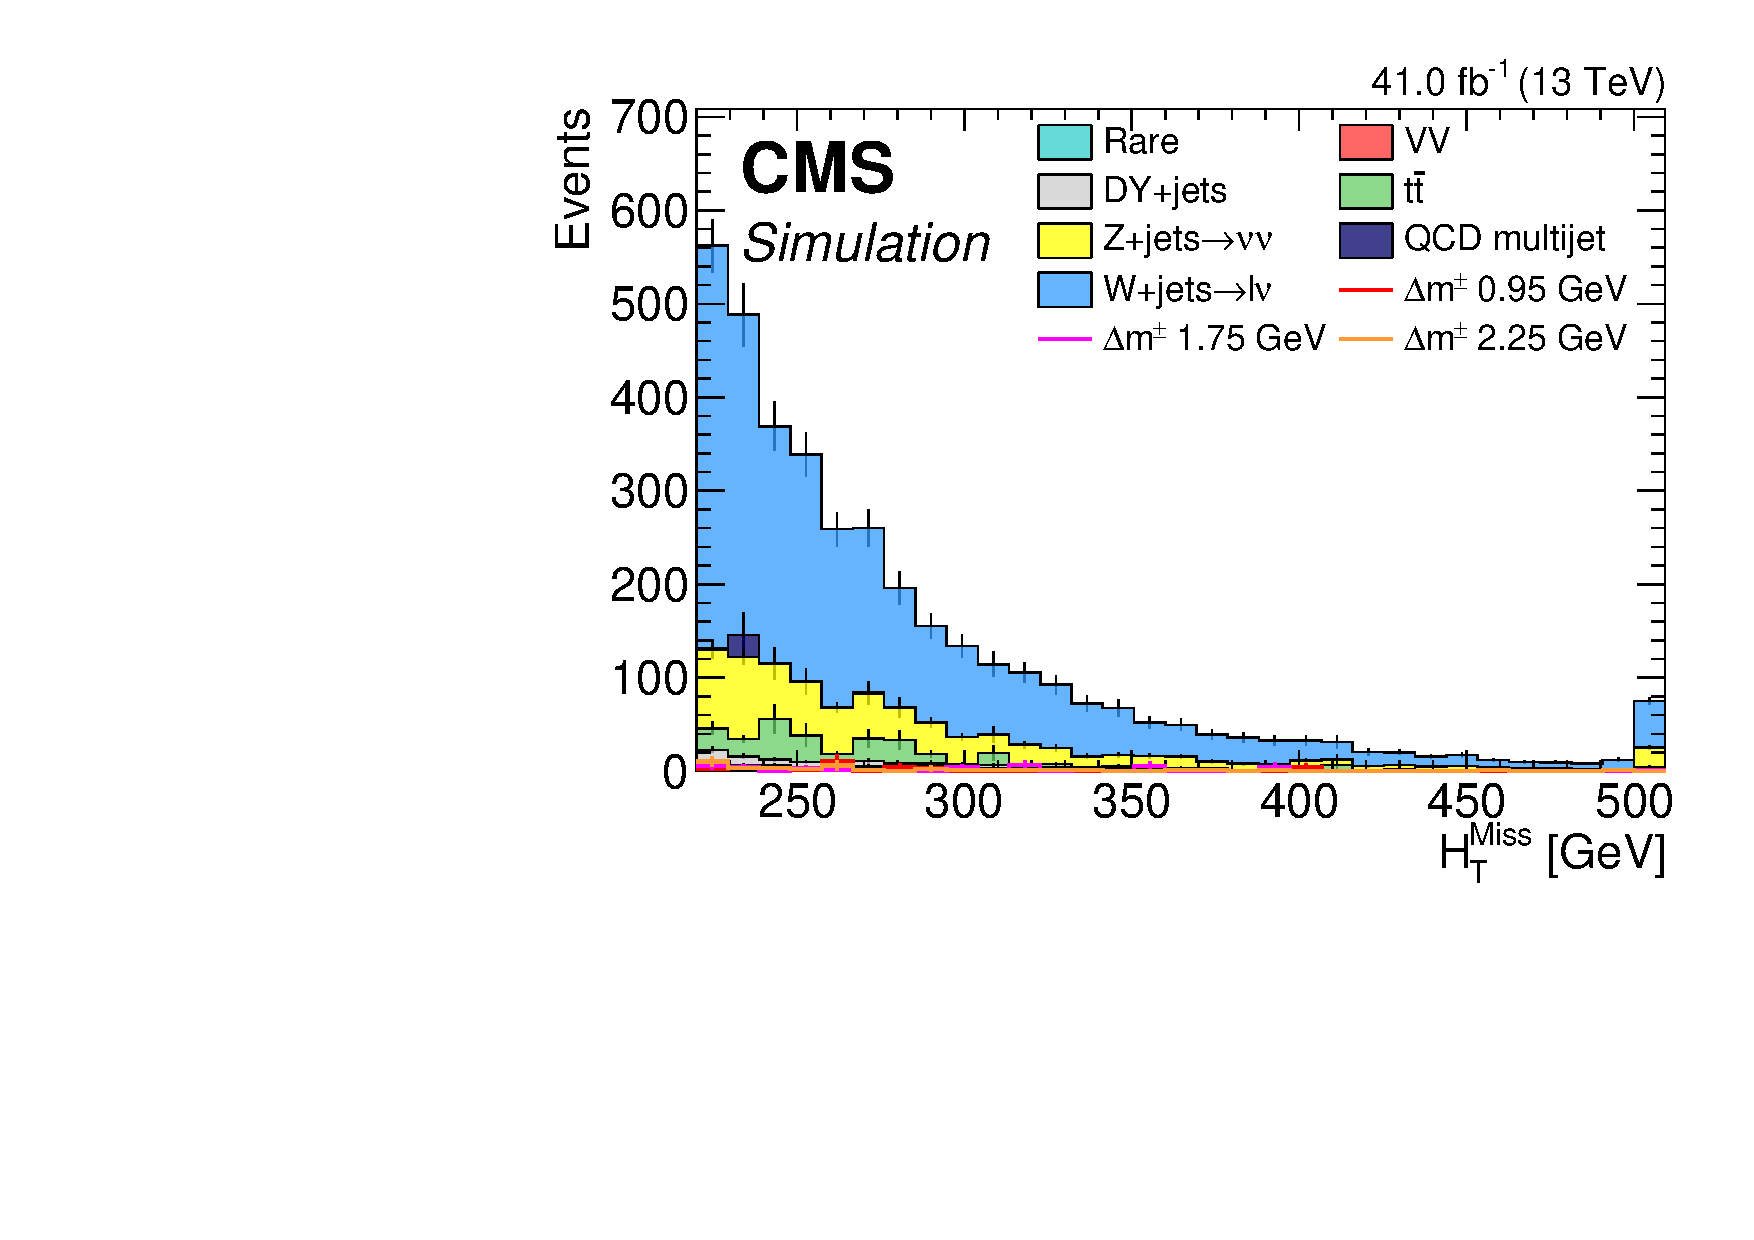
\includegraphics[width=0.48\linewidth]{plots/track_muon_bg_signal/none_MHT.pdf} \,
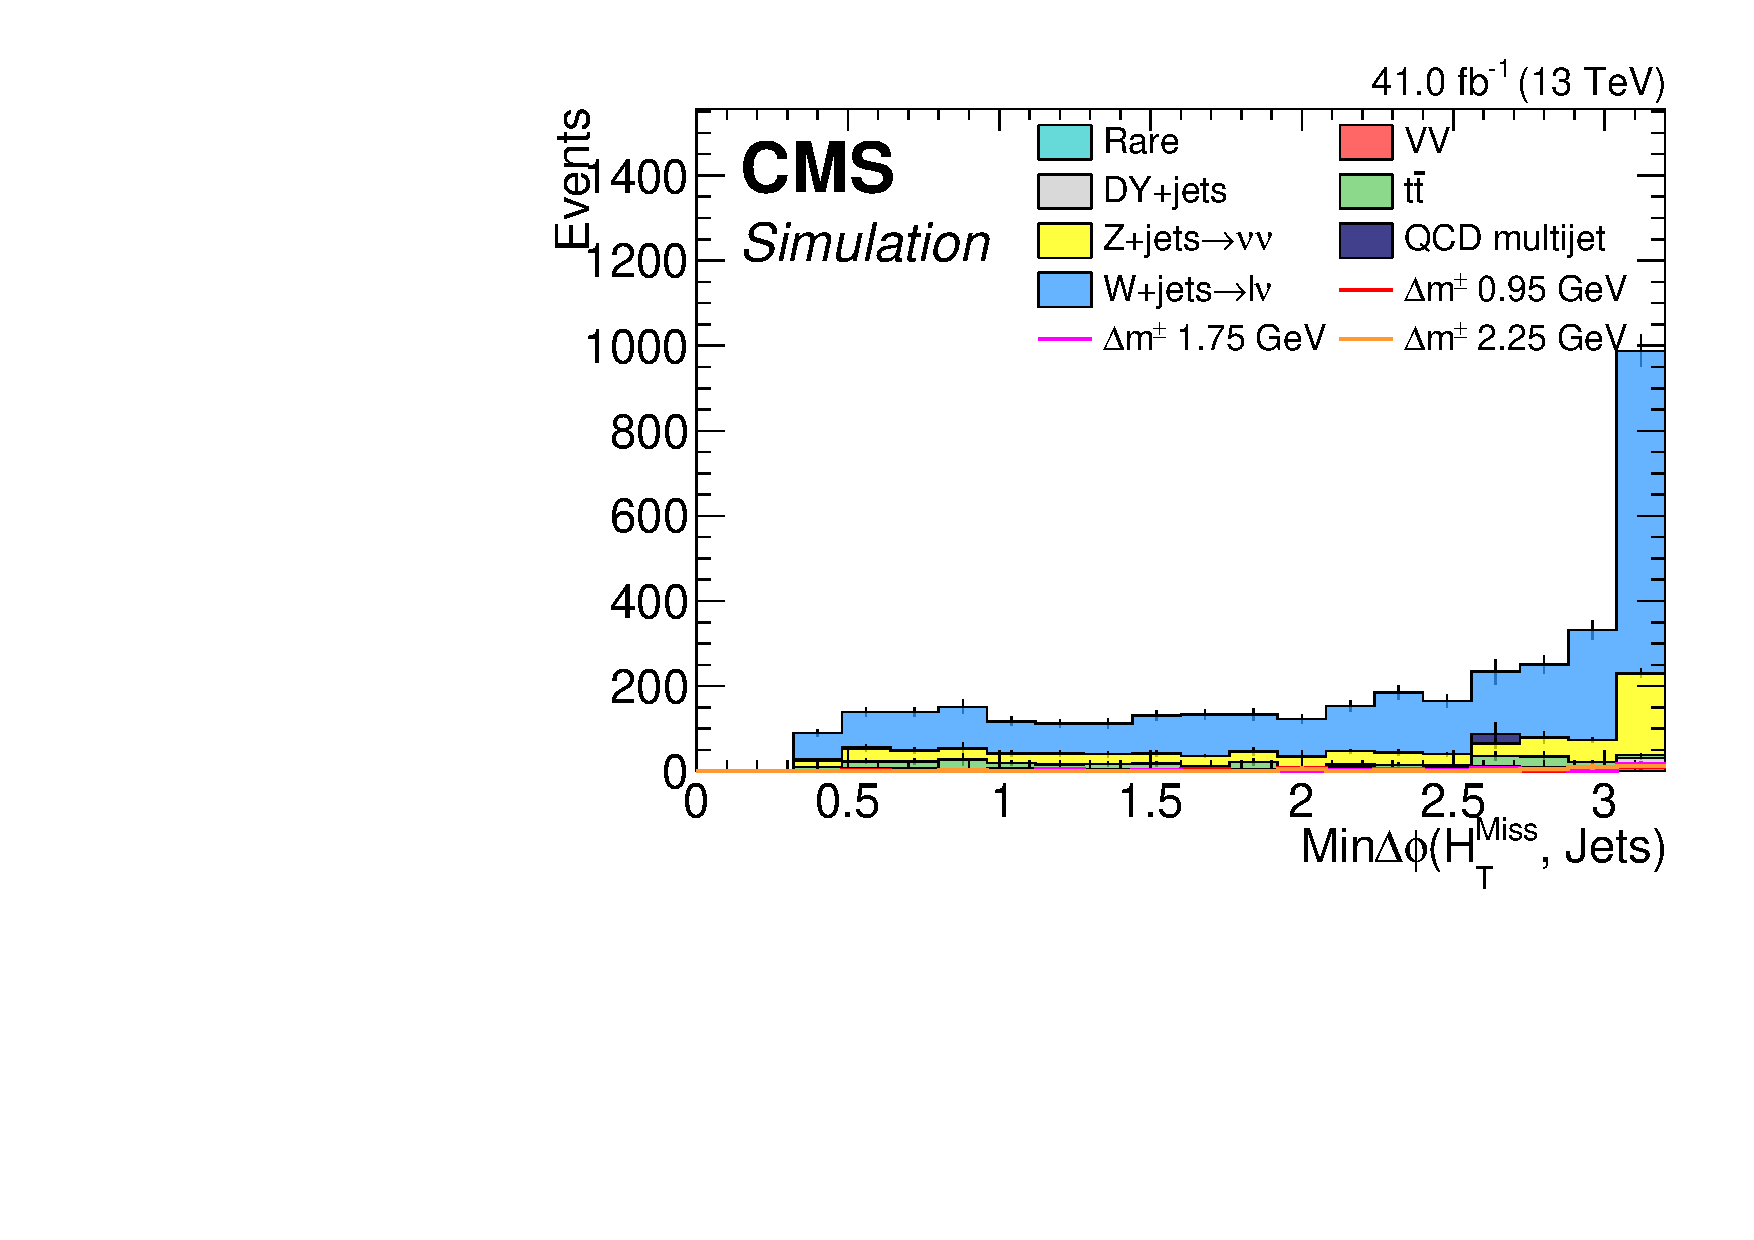
\includegraphics[width=0.48\linewidth]{plots/track_muon_bg_signal/none_MinDeltaPhiMhtJets.pdf} \\
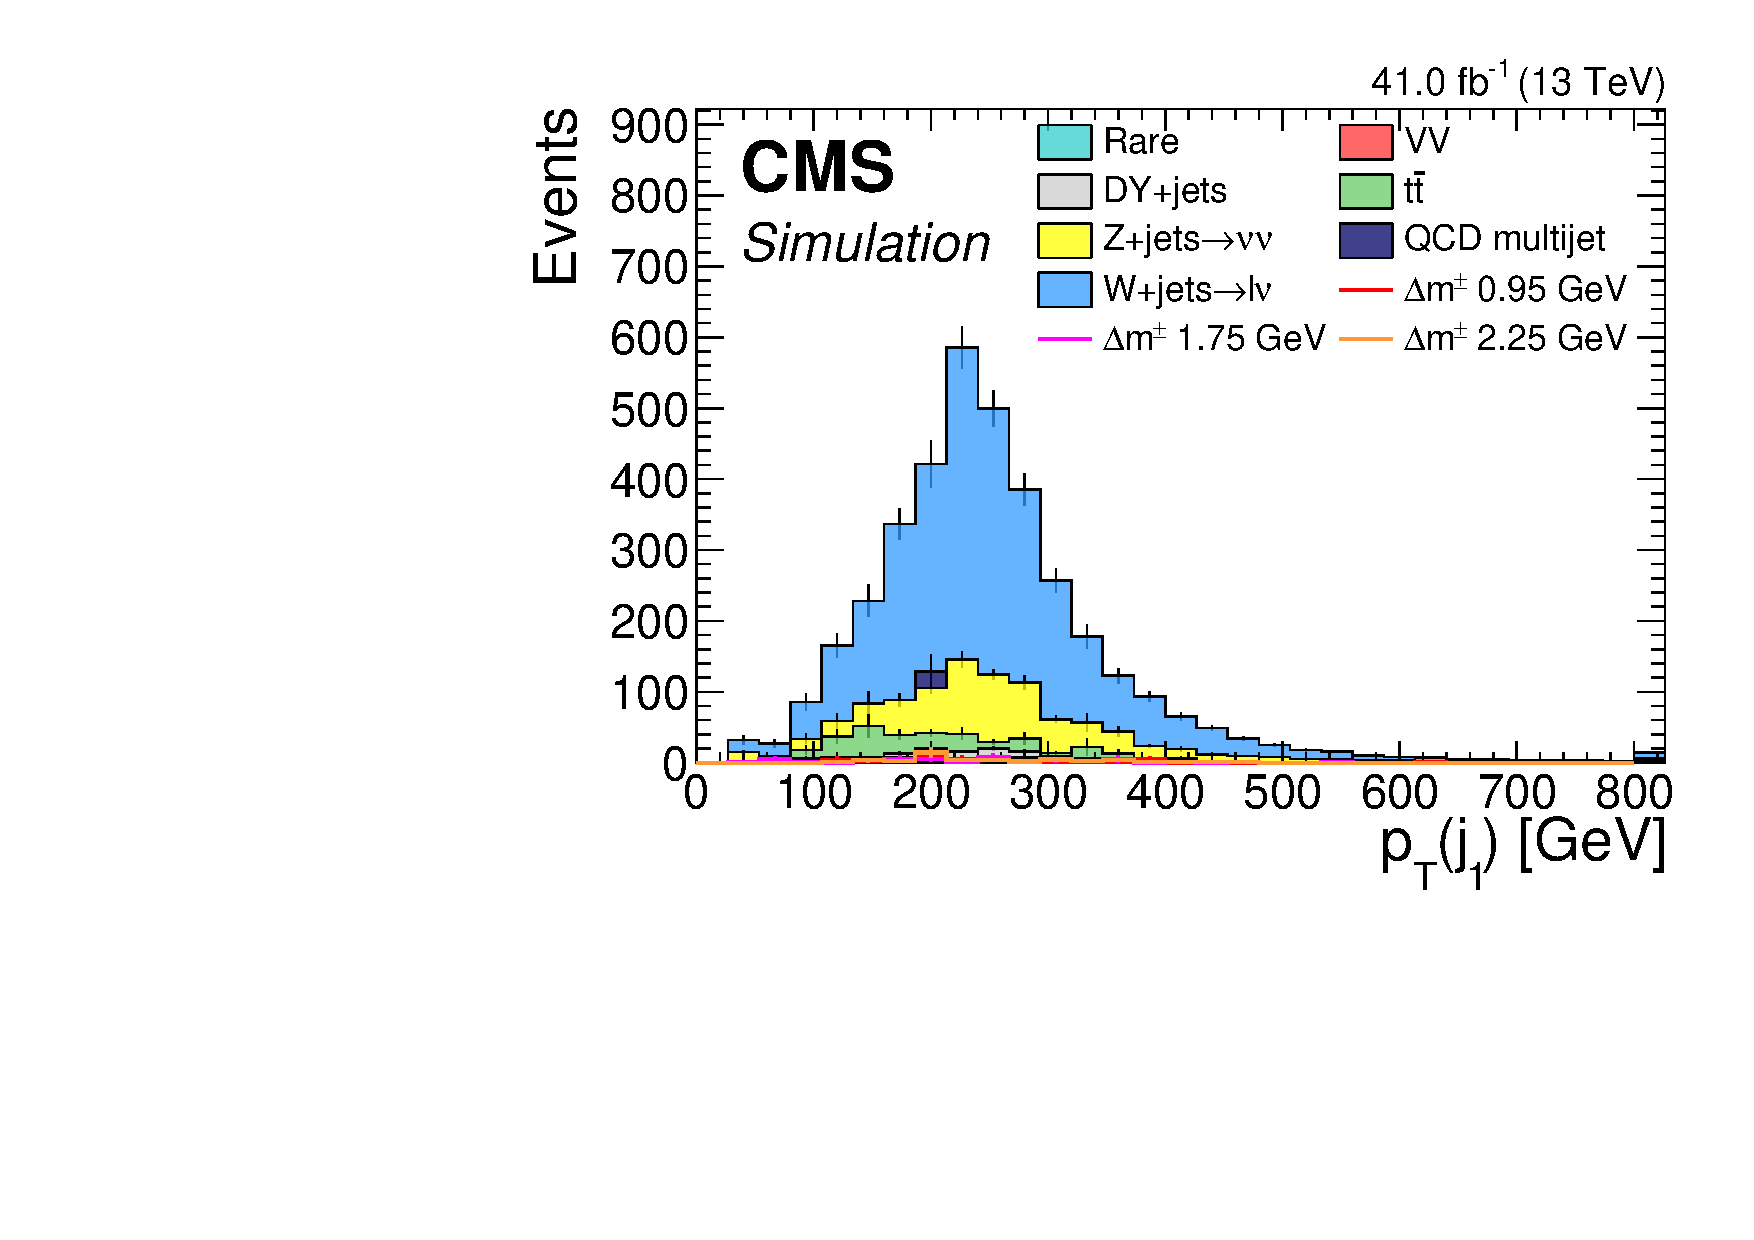
\includegraphics[width=0.48\linewidth]{plots/track_muon_bg_signal/none_LeadingJetPt.pdf} \,
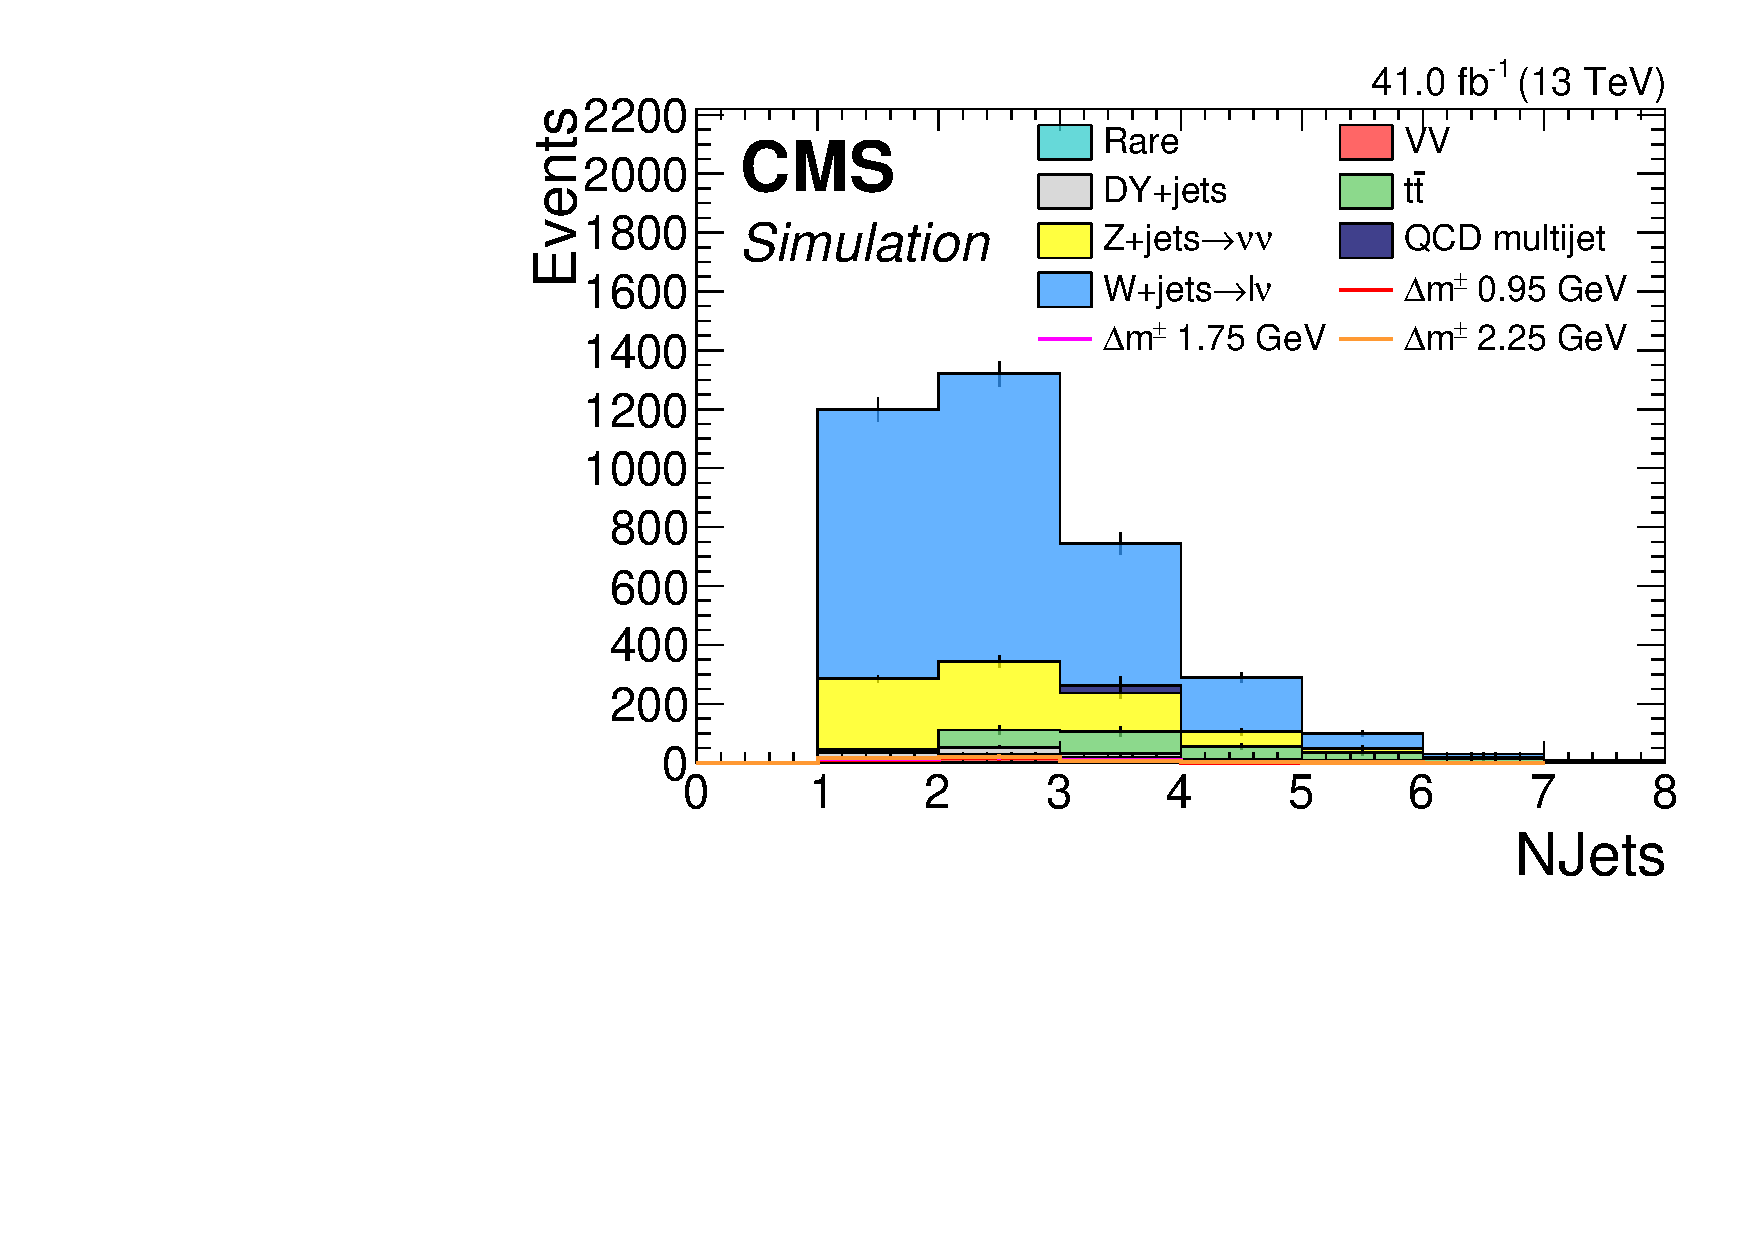
\includegraphics[width=0.48\linewidth]{plots/track_muon_bg_signal/none_NJets.pdf} \\
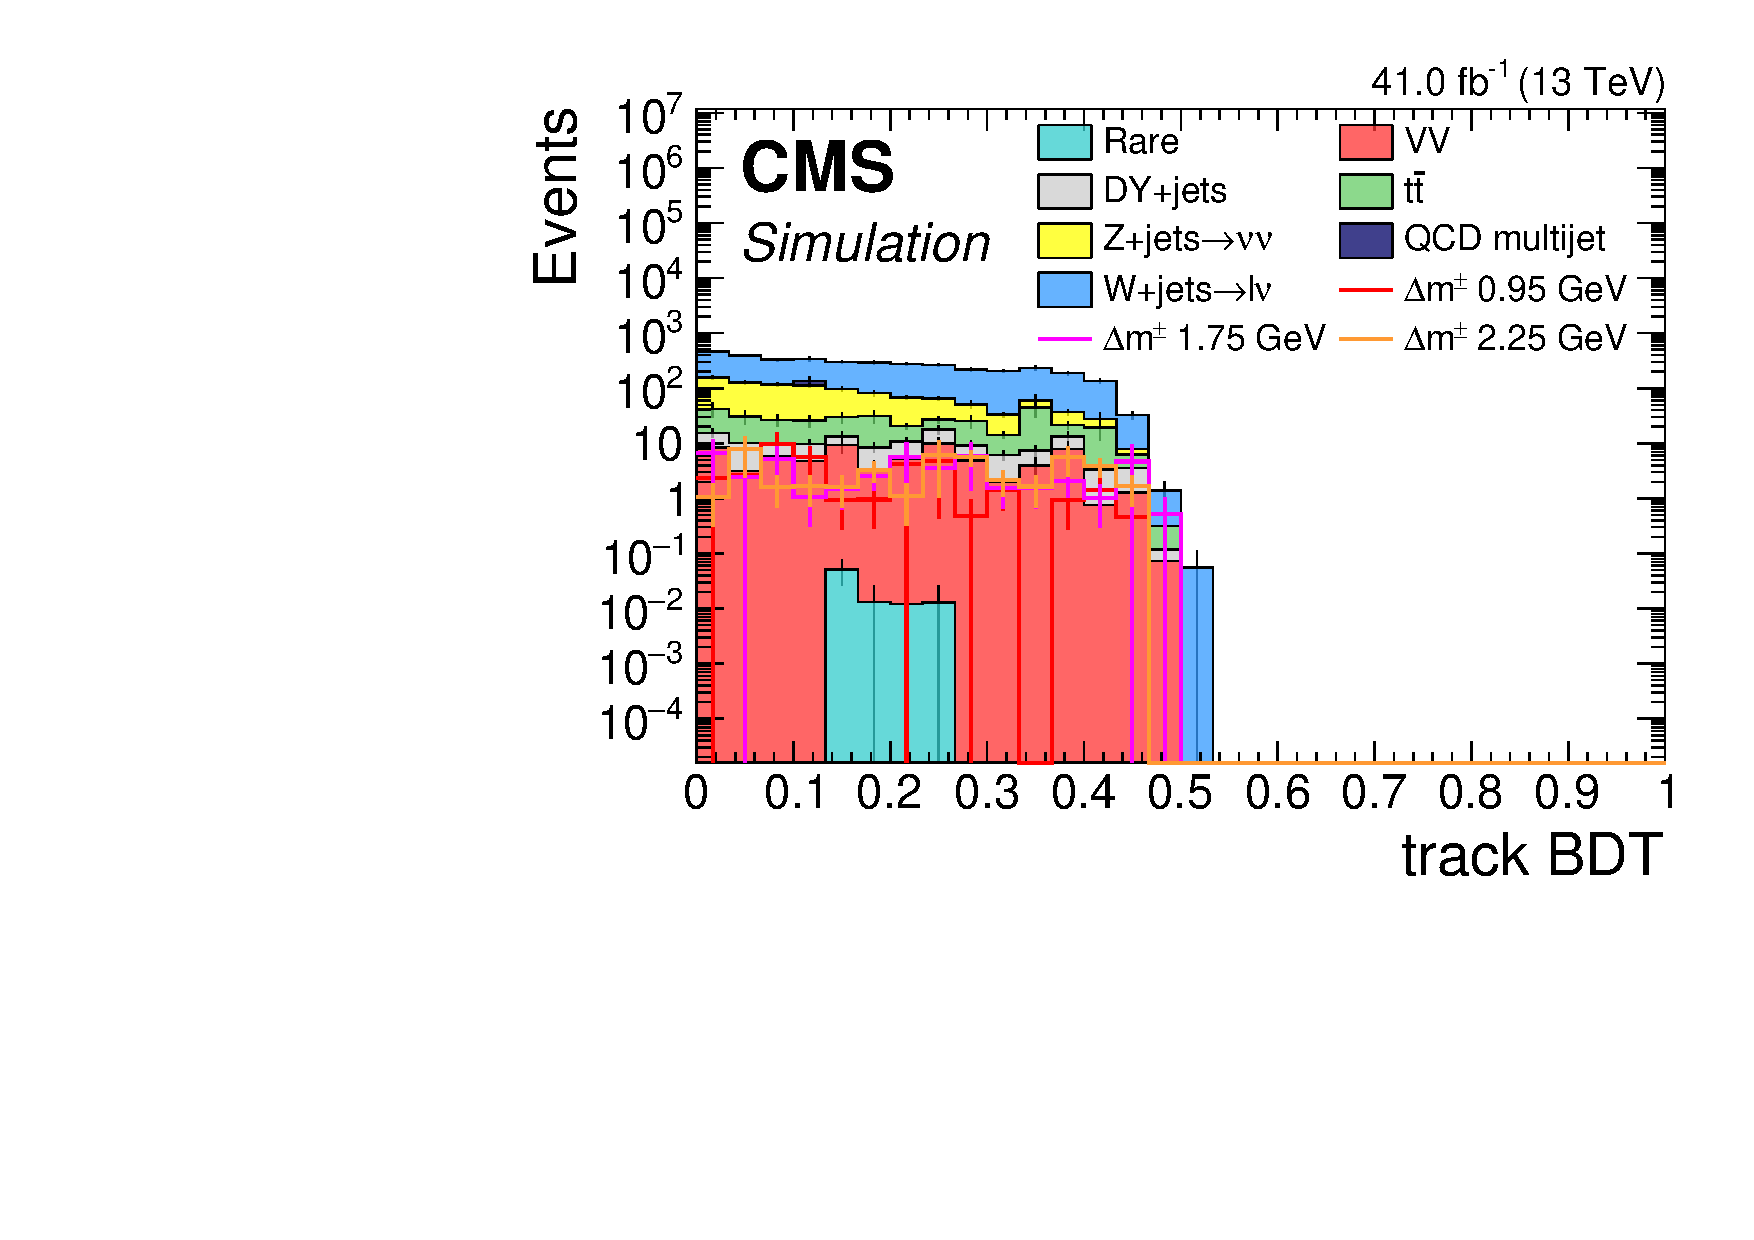
\includegraphics[width=0.48\linewidth]{plots/track_muon_bg_signal/none_trackBDTCorrJetNoMultIso10Dr0.6_log.pdf} \,
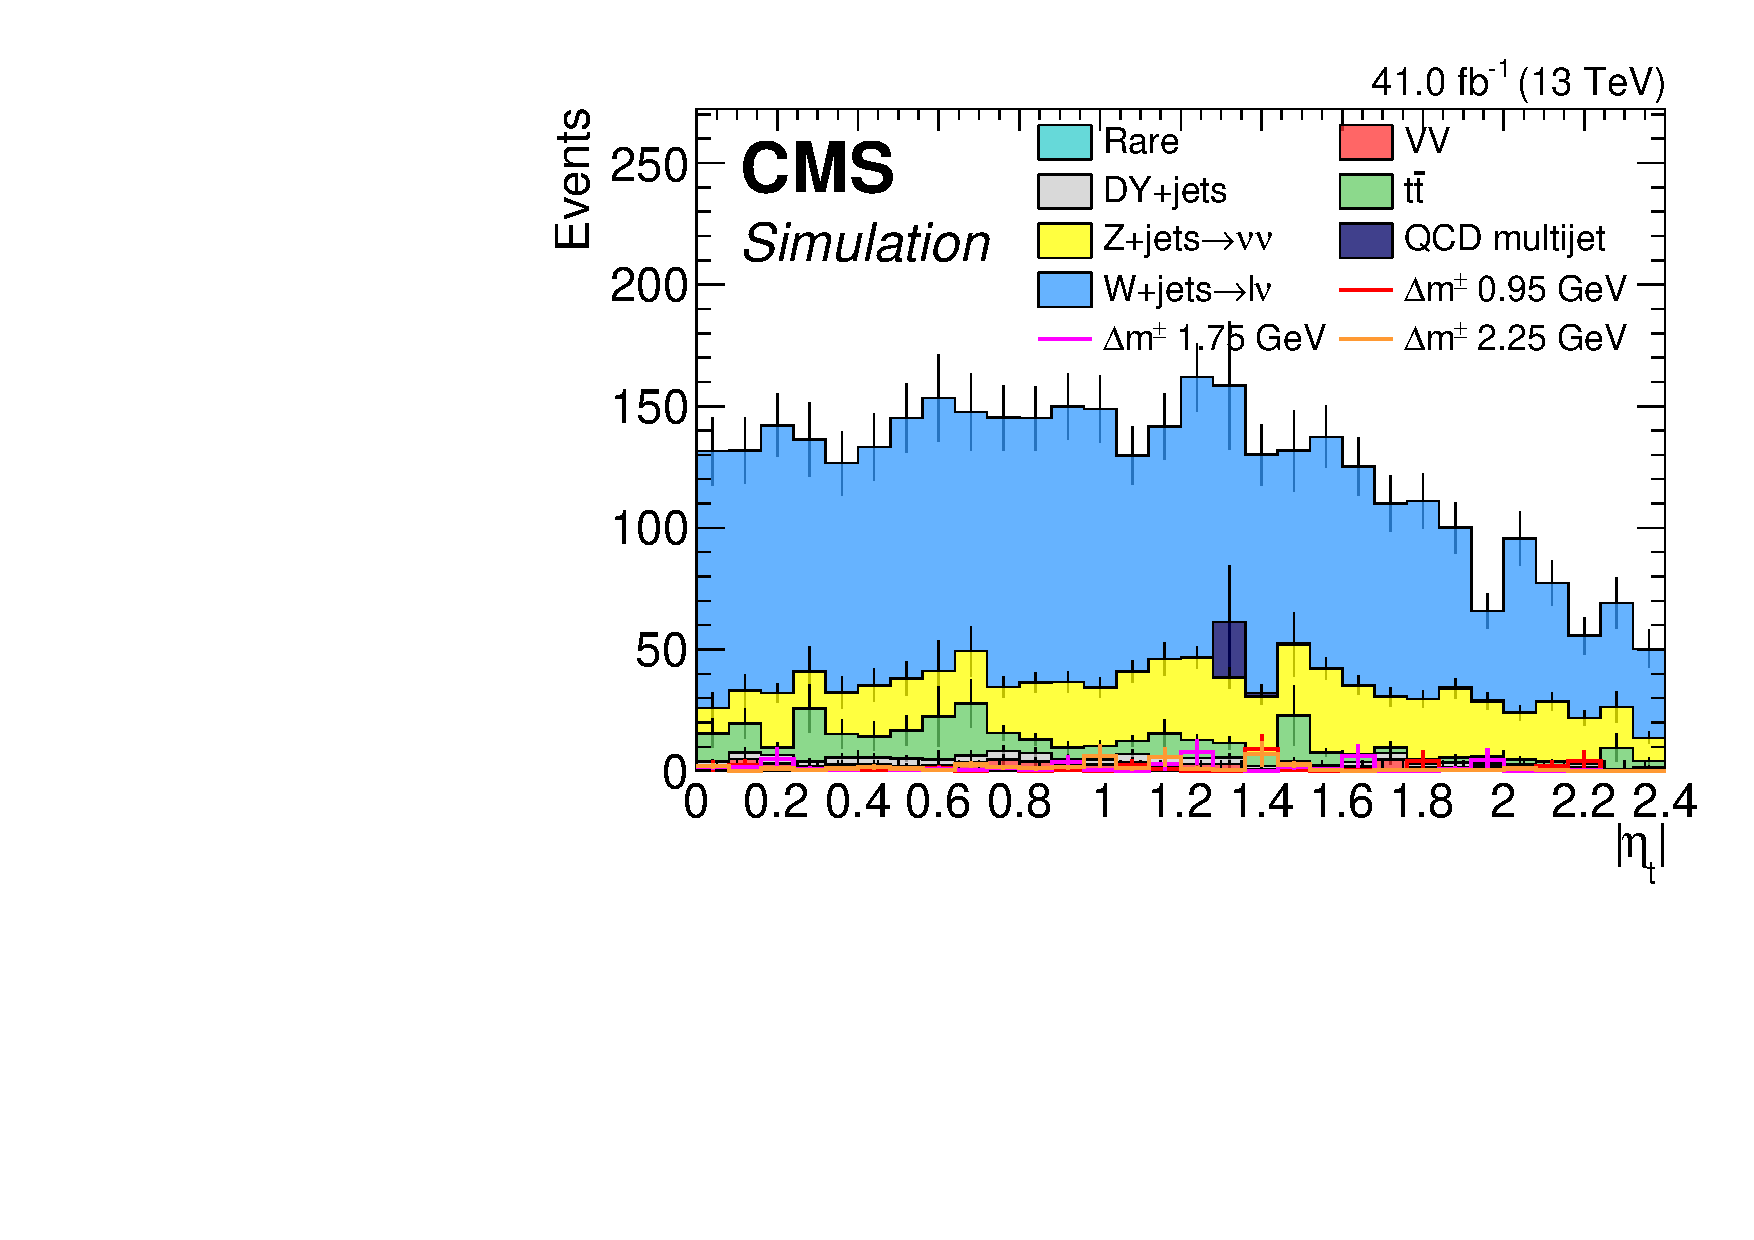
\includegraphics[width=0.48\linewidth]{plots/track_muon_bg_signal/none_abs(trackCorrJetNoMultIso10Dr0.6.Eta()).pdf} \\



\caption[Exclusive track plus muon simulation BDT inputs]{Exclusive track plus muon 2017 simulation BDT inputs for the top 8 ranked observables.}
\label{fig:exclusive-track-muon-bdt-sim-inputs}
\end{figure}


\clearpage
\subsection{Estimation of the Standard Model backgrounds}
\label{sec:background-estimation}

Accurately predicting the event counts for the Standard Model background is one of the central challenges of the analysis. A widely used method for predicting background counts is \gls{mc} simulation. \gls{mc} are weighted to account for production cross-sections and luminosity, and additional correction factors and weights may apply to account for measurement errors, discrepancies between data, and other factors.

Using simulation to estimate the Standard Model background has limitations and disadvantages that can be specific to a given analysis, and depend on the background process under consideration as well as on the observables used in the analysis. The main limitation of simulation is its imperfection. Simulation can never precisely simulate real data due to several factors. Theoretical uncertainties, such as uncertainties on cross sections or branching fractions, can lead to incorrect production rates or normalization. To remedy such effects, simulation is often reweighted using one or more weights derived from a dedicated \gls{cr}. Another challenging limitation of simulation is its likely misrepresentation of the delicate details of a detector’s geometry and response, as well as real-time data-taking conditions which may have varied dynamically throughout a given Run. Some objects and regions of phase space are more prone to discrepancies than others. Using simulation is a reliable method for predicting backgrounds, in which the physics involved has been shown to replicate real data after applying correction factors. In this analysis, the isolated background resulting from the \ztautau process is estimated using simulation. However, due to the imperfect modeling of jets in \gls{mc}, the non-isolated background is modeled using a data-driven method.

A significant challenge arises from the soft nature of the leptons, with low transverse momentum (\pt) and low invariant mass of the order of a few\GeV. The sources of background for such events in the standard model include low-\pt resonances produced in hadronization processes, and events where one of the leptons or exclusive tracks is misidentified as one of the signal leptons. These leptons or tracks are often in close proximity to jets in the event. The analysis uses two strategies to estimate this type of background, depending on whether two identified leptons are present, as in the dimuon category, or only one, as in the exclusive track category. The jetty background estimation for the dimuon category is described in Section~\ref{sec:jetty-background-estimation}, while the exclusive track background estimation is described in Section~\ref{sec:ex-track-background-estimation}. As described earlier, a small portion of the background, namely \ztautau, corresponds to isolated leptons which more closely resemble signal, and the method for estimating this background is described in Section~\ref{sec:mtautau-background-estimation}.

\clearpage
\subsubsection{Jetty background estimation}
\label{sec:jetty-background-estimation}

As discussed in Section~\ref{sec:object-selection}, the leptons in the signal are well isolated. The isolation criterion developed for this analysis is the jet-based isolation described in Section~\ref{sec:isolation}. This customized isolation is also a key part of the background estimation, which is described in this section. This background estimation method applies only to the dimuon category, and its estimated contribution is the largest among the two background processes. It is a \emph{data-driven} background estimation method, meaning that the real data, rather than simulation, are used to estimate this background. The name \emph{non-isolated jetty background} refers to the background in which one or both of the leptons are produced in association with jets and are typically in the angular vicinity of a jet. Most of these leptons are rejected by the jet-isolation criteria, but some do manage to pass the isolation if produced far enough from a jet.

This method uses a sideband \gls{cr} defined by inverting the isolation criteria required for the \gls{sr} to extract a template that is consistent with the shape of the classifier distribution for the jetty background in the \gls{sr}. Separate normalization CR, defined in the negative BDT score region, is used to correct for the different production rates of jetty background in the sideband and main band.

The \gls{sr} is defined by taking BDT output greater than 0, and therefore, by definition, the region with less than 0 becomes a \gls{cr}. The template extraction region is referred to as the \emph{isolation sideband}. The region defining the \gls{sr} with the nominal isolation criteria applied is referred to as the isolation \emph{main band}. The \glspl{sr} are then bins in the isolation \emph{main band} with BDT output greater than zero. The events in the \emph{isolation sideband} are used to predict the jetty-background in the \emph{main band}. The \emph{normalization region} is taken to be in the \gls{cr} with $\mathrm{BDT}<0$, and can also be referred to as the BDT \emph{sideband} or, more elaborately, the \emph{BDT normalization sideband}. Of course though, a \emph{sideband} is still a type of \gls{cr}.

Lepton candidates in the isolation sideband are by definition within an angular distance $\DR$ of 0.6 from a lepton-corrected jet. Any jet causing the lepton to fail the jet-based isolation is required to have an original transverse momentum, i.e., transverse momentum before the lepton momentum subtraction, satisfying $15<\pt<30\GeV$. The upper bound of $30\GeV$ is chosen because this is the lower bound on the analysis jets, effectively decorrelating the isolation observable from the \mht and the number of jets in the event. In the absence of such of an upper bound, a bias in the isolation sideband could, for example, be introduced because requiring a lepton to fail jet-based isolation would require the presence of an additional analysis jet, which is not the case in the main band. The BDT is also not sensitive to these softer jets, and so the shape of the classifier score distribution in the sideband should be unaffected by the isolation requirement, resulting in consistent shapes between the main band and the sideband.

The main assumption underpinning the use of the isolation sideband is that, in the jetty background, the leptons are not isolated but are created in association with jets. Most of them are produced inside the jets, with a distribution that falls off as a function of the angular distance $\DR$ to jet. By selecting leptons inside the cone around the soft jet, events are picked up that have similar behavior to events where the leptons are outside of those cones. The rate of lepton production inside jets differs from those outside jets, but much about the object and event kinematics is well-matched between the sideband and main band, and only a normalisation correction factor must be applied to bring the two shapes into statistical agreement. The normalization factor is derived by taking the ratio between the event count in the main band and that in the isolation sideband in the normalisation CR, defined in the region with BDT score less than 0. The event counts in the sideband are then scaled by the normalization factor to make up the prediction. The prediction in the \gls{sr} then becomes:
\begin{equation}
\hat{\mathrm{N}}^{\mathrm{SR}}_{\text{jetty}} = \frac{\mathrm{N}^{\text{norm CR}}_{\text{main band}}}{\mathrm{N}^{\text{norm CR}}_{\text{sideband}}} \cdot\mathrm{N}^{\mathrm{SR}}_{\text{sideband}},
\end{equation}
where the transfer factor is:
\begin{equation}
\hat{\mathrm{TF}}_{\text{jetty}} = \frac{\mathrm{N}^{\text{norm CR}}_{\text{main band}}}{\mathrm{N}^{\text{norm CR}}_{\text{sideband}}}.
\end{equation}
The transfer factors are listen in Table~\ref{tab:transfer-factors}.


To test the assumption that the isolation sideband, \ie, events with at least one of the leptons failing the jet isolation criterion, correctly predicts the shape of the main band in the signal region, a shape comparison is performed in simulation. This shape comparison, also known as a \emph{closure test}, is carried out by evaluating the consistency of the ratio between the predicted and direct MC values with unity. A normalization factor is computed to correctly normalize the isolation sideband. This is ultimately the same procedure carried out on data to derive the data-driven predictions. This section presents the Phase 1 closure test, carried out using 2017 \gls{mc}. An additional correction has been carried out in the case of Phase 0, which is discussed in Section~\ref{sec:systematic-uncertainties}.

\begin{figure}[!htb]
\centering
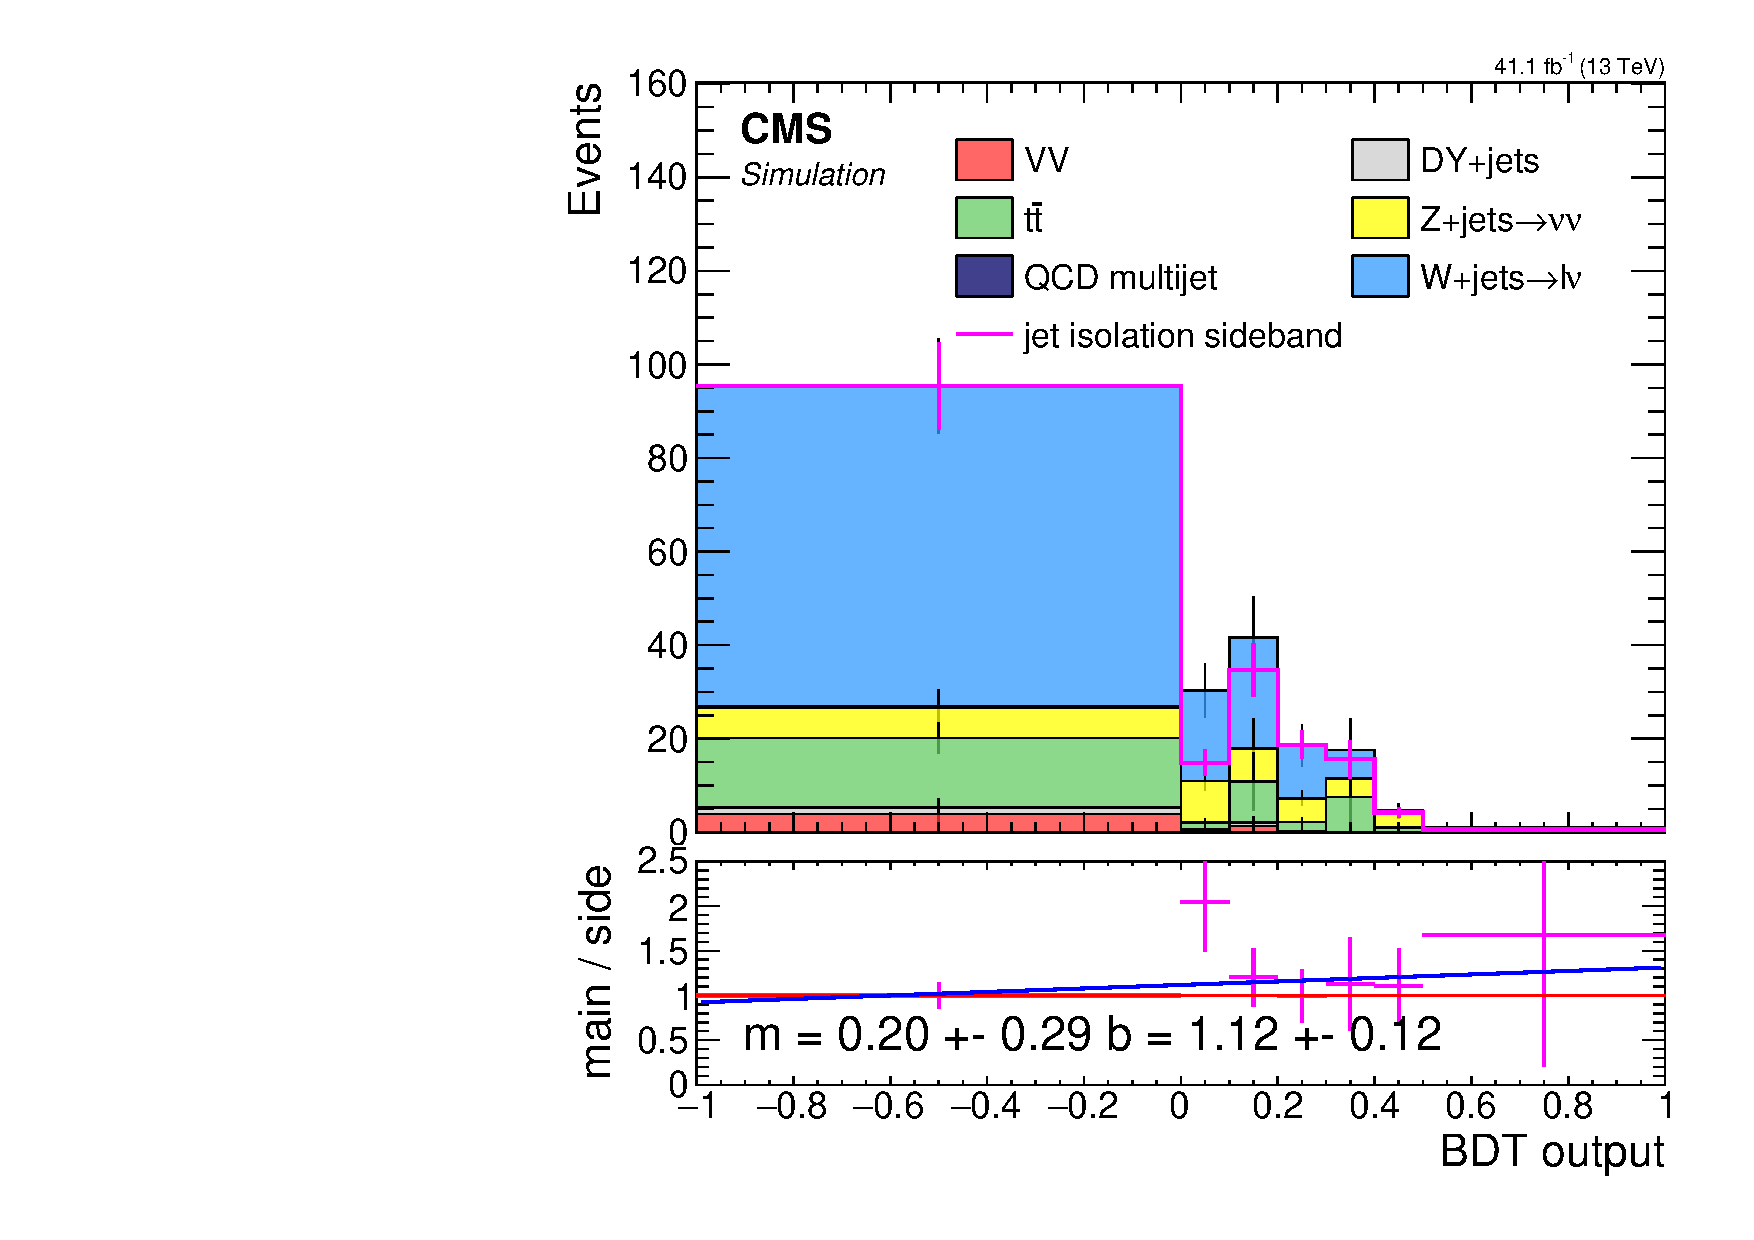
\includegraphics[width=0.60\linewidth]{plots/dilepton_muons_2017_closure/none_closure_dilepBDTphase1CorrJetNoMultIso10Dr0.6.pdf}  \\


\caption[Event distributions comprising the Phase 1 jetty background closure test.]{Event distributions comprising the Phase 1 jetty background closure test. The stack represents simulation in the isolation main band, \ztautau not included, while the pink line represents simulation in the isolation sideband scaled by the normalisation correction factor $\hat{\mathrm{TF}}_{\text{jetty}}$. The lower panel shows the ratio between the isolation main band and sideband. A line fit of the ratio is performed and the parameters of the slope $m$ and interception point $b$ with their respective errors are printed.}
\label{fig:dimuon-bdt-jetty-2017-closure}
\end{figure}

Figure~\ref{fig:dimuon-bdt-jetty-2017-closure} shows the results of the jetty background closure test. The overall shapes are compatible, and the trend line is statistically compatible with a horizontal line at unity, and most bins are statistically consistent with 1. The trend line indicates there is no need for for additional correction, but the uncertainty in the trend line constitutes the basis of a systematic uncertainty in the shape of the isolation sideband template. The full list of transfer factors with the associated uncertainties can be found in Section~\ref{sec:data-driven-tranfer-factors}, while the special treatment of the 2016 case is discussed in Section~\ref{sec:data-driven-shape}.

\clearpage
\subsubsection{Ditau Drell-Yann background estimation}
\label{sec:mtautau-background-estimation}

A small amount of background arising from \ztautau is also present in the SR, which is the only identified background not accounted for by the jetty method. Since the leptons resulting from the leptonic decay \tautomu are isolated, it requires an alternative background estimation method.

The \ztautau background is estimated using \gls{mc} simulation weighted according to a data-to-MC correction factor computed in a dedicated \gls{cr} that is relatively pure in \ztautau background. This control region is constructed by placing requirements on the observable \mtautau, explained below. If the taus could be fully reconstructed, their system invariant mass \mtautau would peak around the \PZ mass. The \PZ resonance could then be used as the desired \gls{cr} rich in ditau background. However, since leptonic taus are not directly reconstructed, an alternative approach must be formulated.

A widely used method for the reconstruction of the invariant mass \mtautau is the \emph{collinear approximation}. First described in~\cite{ELLIS1988221_first_mtautau}, it has been used in \acrshort{atlas}~\cite{ATLAS:2009zsq} and \acrshort{cms}~\cite{CMS:2007sch}. In this approximation, it is assumed that each $\PGt$ produced from \PZGammaStar is highly energetic, such that its decay products are collinear, and that the source of missing transverse momentum is the neutrinos. If both $\PGt$-leptons are sufficiently boosted, the neutrinos from each $\PGt$ decay are collinear with the visible lepton momentum. The visible daughter-lepton momentum is used together with \VEtmiss to reconstruct the $\PGt$-lepton pair and calculate the invariant mass. Depending on the details of the approximation, one can arrive at a strictly positive distribution for \mtautau, as in~\cite{Han_2014_positive}, or one that also has negative values as in~\cite{Baer_2014_negative,Barr_2015_diff}. The negative values correspond to events where \VEtmiss points more than 90 degrees in $\phi$ from one of the leptons, which is not consistent with with the topology of boosted ditau events, and thus it is useful to reject negative values in order to purify the \gls{cr}. The collinear approximation breaks down when the $\PGt$s are back-to-back. However, since in the analysis presented in this thesis requires a high-\pt jet and large \MET, he considered event topology yields results in sensible values. The signal, as well as other SM processes, are expected to have a smooth and relatively flat distribution in \mtautau, while events arising due to \ztautau are expected to peak around the \PZ boson mass.

To illuminate the logic behind this observable, the following is a derivation of \mtautau approximation. The invariant mass is defined as:
\begin{equation}
\label{eq:mtautau}
\mtautau^2 = (p_{\PGt_1} + p_{\PGt_2})^2.
\end{equation}
Assuming that the $\PGt$-pair is boosted and the fully leptonic decay products are fully collinear to the $\PGt$-leptons, it follows that the transverse momentum of each neutrino pair is proportional to the corresponding $\PGt_i$'s transverse momentum by a scale factor $\xi_i$:
\begin{equation}
\vec{\pt}^{\PGn_i}=\xi_i \vec{\pt}^{\PGt_i}.
\end{equation}
Since by assumption, all of the missing transverse momentum is due to the neutrinos, and therefore it follows that
\begin{equation}
\label{eq:two-mtautau}
\ptvecmiss =\xi_1 \vec{\pt}^{\PGt_1}+\xi_2 \vec{\pt}^{\PGt_2}.
\end{equation}
Solving the above two equations~\ref{eq:two-mtautau} for the two parameters $\xi_1$ and $\xi_2$ for each event, the solution becomes:
\begin{equation}
\begin{split}
\xi_1 = \frac{{{\vec p}_{\mathrm{T}_x}^{\kern1pt\text{miss}}} \cdot {\vec p}_y^{\ell_2}  - {{\vec p}_{\mathrm{T}_y}^{\kern1pt\text{miss}}} \cdot {\vec p}_x^{\ell_2}  }{ {\vec p}_{x}^{\ell_1} \cdot {\vec p}_{y}^{\ell_2} -  {\vec p}_{x}^{\ell_2} \cdot {\vec p}_{y}^{\ell_1} },\\
\xi_2 = \frac{{{\vec p}_{\mathrm{T}_y}^{\kern1pt\text{miss}}} \cdot {\vec p}_x^{\ell_1}  - {{\vec p}_{\mathrm{T}_x}^{\kern1pt\text{miss}}} \cdot {\vec p}_y^{\ell_1}  }{ {\vec p}_{x}^{\ell_1} \cdot {\vec p}_{y}^{\ell_2} -  {\vec p}_{x}^{\ell_2} \cdot {\vec p}_{y}^{\ell_1} }.
\end{split}
\end{equation}
Equation~\ref{eq:mtautau} is expanded based on the assumption that the $\PGt$'s are boosted and that the four-momenta of the $\PGt$s is $p_{\PGt_i} = (1+\xi_i)p_{\ell_i}$:
\begin{equation}
\label{eq:mtautau-approx}
\begin{split}
\mtautau^2 &= ({p_\PGt}_1 + {p_\PGt}_2)^2 \\
&=\left((1+\xi_1){p_\ell}_1+(1+\xi_2){p_\ell}_2\right)^2\\
&=2m_\PGt^2+2(1+\xi_1)(1+\xi_2){p_\ell}_1\cdot {p_\ell}_2\\
&\approx 2(1+\xi_1)(1+\xi_2){p_\ell}_1\cdot {p_\ell}_2.
\end{split}
\end{equation}
This can be negative if one of the $\xi_i$ satisfy $\xi_i < -1$. This can happen if the missing transverse momentum vector nearly opposite to a lepton's \ptvec and also $\ptmiss > \pt^\ell$. This can easily happen in non-DY processes, such as $\mathrm{WW}$+jets , when a neutrino and a lepton (possibly coming
from different decay legs) are nearly back-to-back. Therefore, the final definition of \mtautau is
\begin{equation}
\mtautau = \mathrm{sign}(\mtautau^2)\sqrt{\abs{\mtautau^2}}.
\end{equation}

The \gls{cr} constructed to constrain the \ztautau background should have high purity, and thus minimal contamination from SUSY signal and other processes. Figure~\ref{fig:dimuon-bdt-sim-output} shows that the region of $\text{BDT} < 0$ has negligible signal contamination, and is therefore used as a starting point to build the \tautau \gls{cr}. Figure~\ref{fig:mtautau-distributions} displays the \mtautau distributions for the \tautau MC in red and the rest of the standard model backgrounds in the stack. The results for the two tracker phases are presented side by side. A clear peak in the \tautau background is observed around the mass of the \PZ boson. A window around the \PZ boson's mass of $[40,130]\GeV$ is chosen to achieve high purity of about 75\% in both phases. Contamination from other backgrounds is removed by first predicting the jetty background count using the data-driven method described in Section~\ref{sec:jetty-background-estimation}, and subtracting those counts from the data counts in the \tautau dedicated \gls{cr}. The ratio of data to MC is extracted from this region, with the result $1.2\pm 0.46$ ($0.29\pm 0.26$), which has a relative error of 38\% (90\%) for Phase 0 (Phase 1).

\begin{figure}[!htb]
\centering
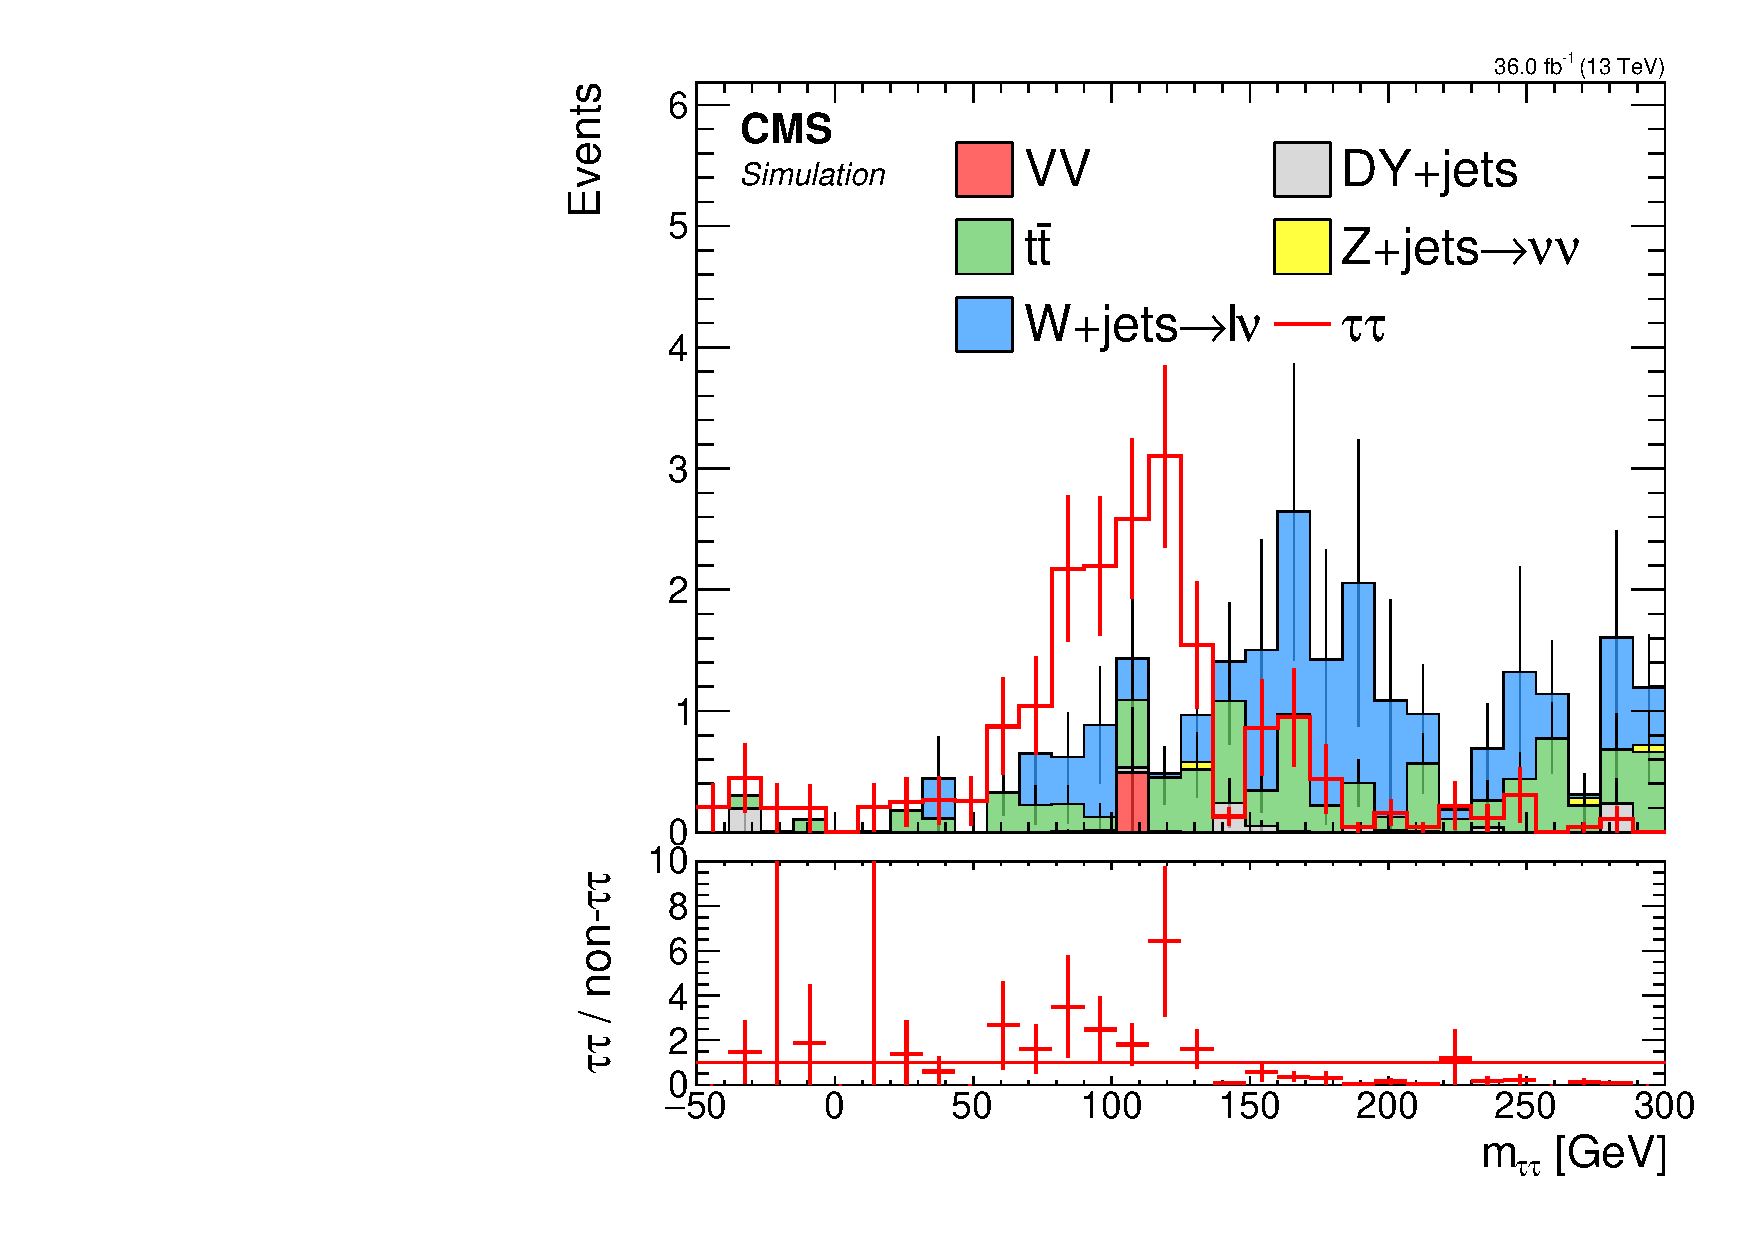
\includegraphics[width=0.48\linewidth]{plots/dilepton_muons_bg_isocr_scan_tautau_vs_no_tautau/bdt2_nmtautauCorrJetNoMultIso10Dr0.6.pdf} \,
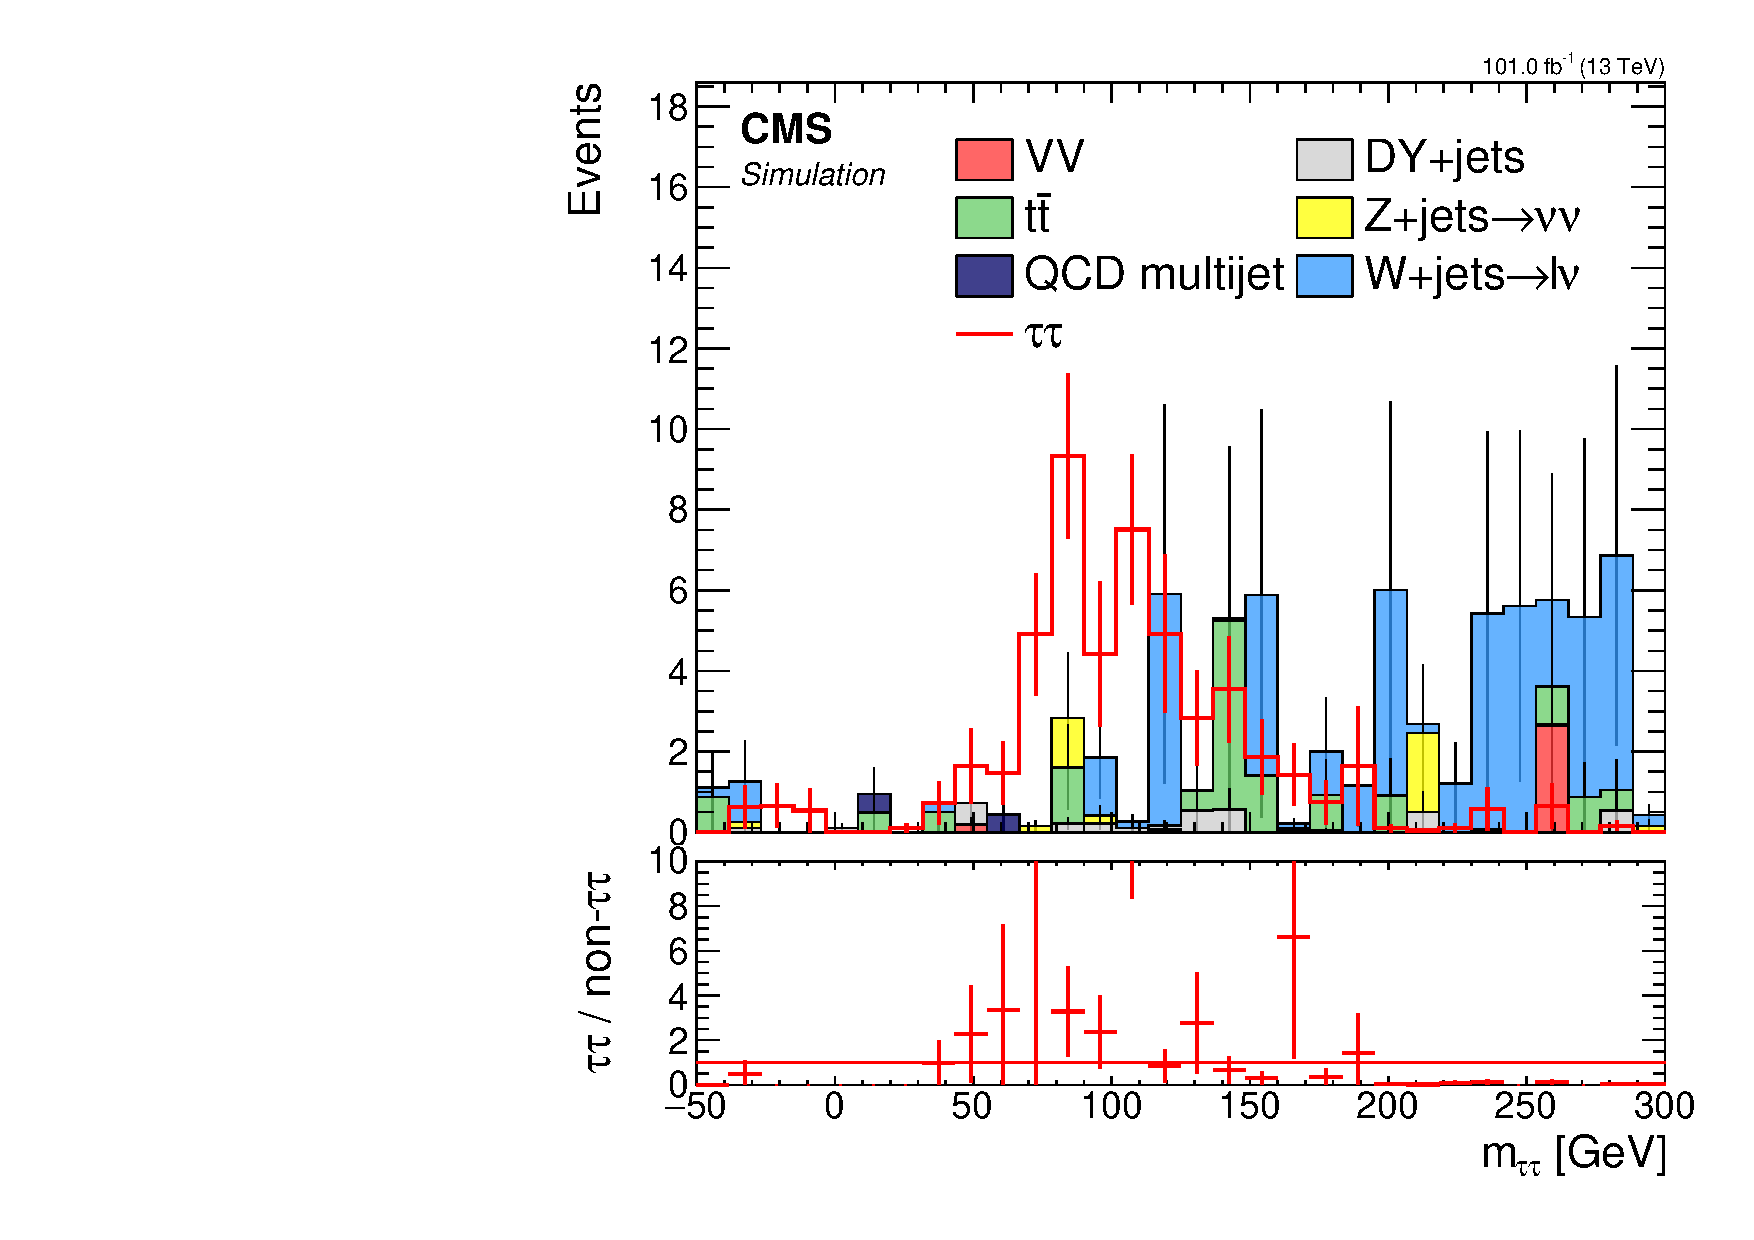
\includegraphics[width=0.48\linewidth]{plots/dilepton_muons_bg_isocr_scan_tautau_vs_no_tautau_phase1/bdt_nmtautauCorrJetNoMultIso10Dr0.6.pdf} \\


\caption[Ditau invariant mass distibutions]{Ditau invariant mass \mtautau distributions for phase 0 2016 simulation (left) and phase 1 2017 simulation weighted to luminosity of 2017-2018 data taking period (right). The red line corresponds to \tautau simulation, and the stack represents the rest of the standard model background simulation. No overflow bins are plotted in order to clearly show the resonance peak.}
\label{fig:mtautau-distributions}
\end{figure}

\clearpage
\subsubsection{Exclusive track background estimation}
\label{sec:ex-track-background-estimation}

The exclusive track category uses four separate \glspl{bdt}, one for each lepton flavor, and for each phase. However, the background estimation method is the same for all of them.

The exclusive track category requires one identified lepton according to the selection listed in Sections~\ref{sec:object-selection-electrons} and~\ref{sec:muon-selection}, and one track selected by a procedure described fully in Section~\ref{sec:track-bdt}. The track is chosen with the highest \gls{bdt} score among all tracks in each event using the track-picking BDT that was trained to pick up the track that corresponds to the non-identified lepton in the signal event. The chance of selecting a track/lepton pair corresponding to the decay of a single resonant particle is vanishingly small. It is highly likely that the track corresponds to an unrelated charged hadron or is a fake track, meaning a fluke in the tracking pattern recognition procedure.

To devise a reliable background estimation procedure for the exclusive track category, a symmetry is exploited relating to the charge of tracks in the background. The nominal selection requires tracks with opposite charge to the identified lepton, but given that the track is produced independently from the lepton, events with a track of the same charge have otherwise practically indistinguishable characteristics from events with opposite charge pairs. Both the overall rate as well as the shape of the \gls{bdt} output are generally equivalent, making it an excellent proxy to the true background.

A \gls{cr} is defined by selecting events with a same-charge lepton-track pair rather than an opposite-charge pair as in the \gls{sr}. Tthe normalization is fixed by calculating a normalization factor as the ratio between the opposite-charge and same-charge event count in a dedicated normalization sideband \gls{cr} satisfying $\text{BDT} < 0$, and applying it to the same-charge event count in the \glspl{sr} satisfying $\text{BDT} > 0$. In order to test the independence assumption and to demonstrate the correct shape and normalization prediction, a closure test is performed using MC data. Figure~\ref{fig:ex-track-closure-tests} shows the results of the closure tests for muons and electrons for both tracker phases. In each plot, the stack represents SM background for the nominal (opposite-charge) analysis selection lepton-track pair (oc), while the orange line represents the same-charge lepton-track pair (sc). In the ratio panel, which shows the ratio between the opposite-charge to same-charge backgrounds for each bin, the shapes of the nominal and sc backgrounds are seen to consistent.

After establishing that the method can be used to correctly predict the background, a data-driven normalization factor is computed as the ratio between opposite-charge to same-charge data event count in the \gls{cr} of $\text{BDT} < 0$. The final prediction in the \glspl{sr} then becomes the same-charge data event count in the \gls{sr} multiplied by the normalization factor.

The computed normalization factor for phase 0 (2016) is $1.12\pm 0.044$ ($1.037\pm 0.05$) for muons (electrons), and for phase 1 (2017-2018) is $1.066\pm 0.024$ ($1.049\pm 0.03$) for muons (electrons). The relative errors on the normalization factors are between 2\% to 5\%.


\begin{figure}[!htb]
\centering
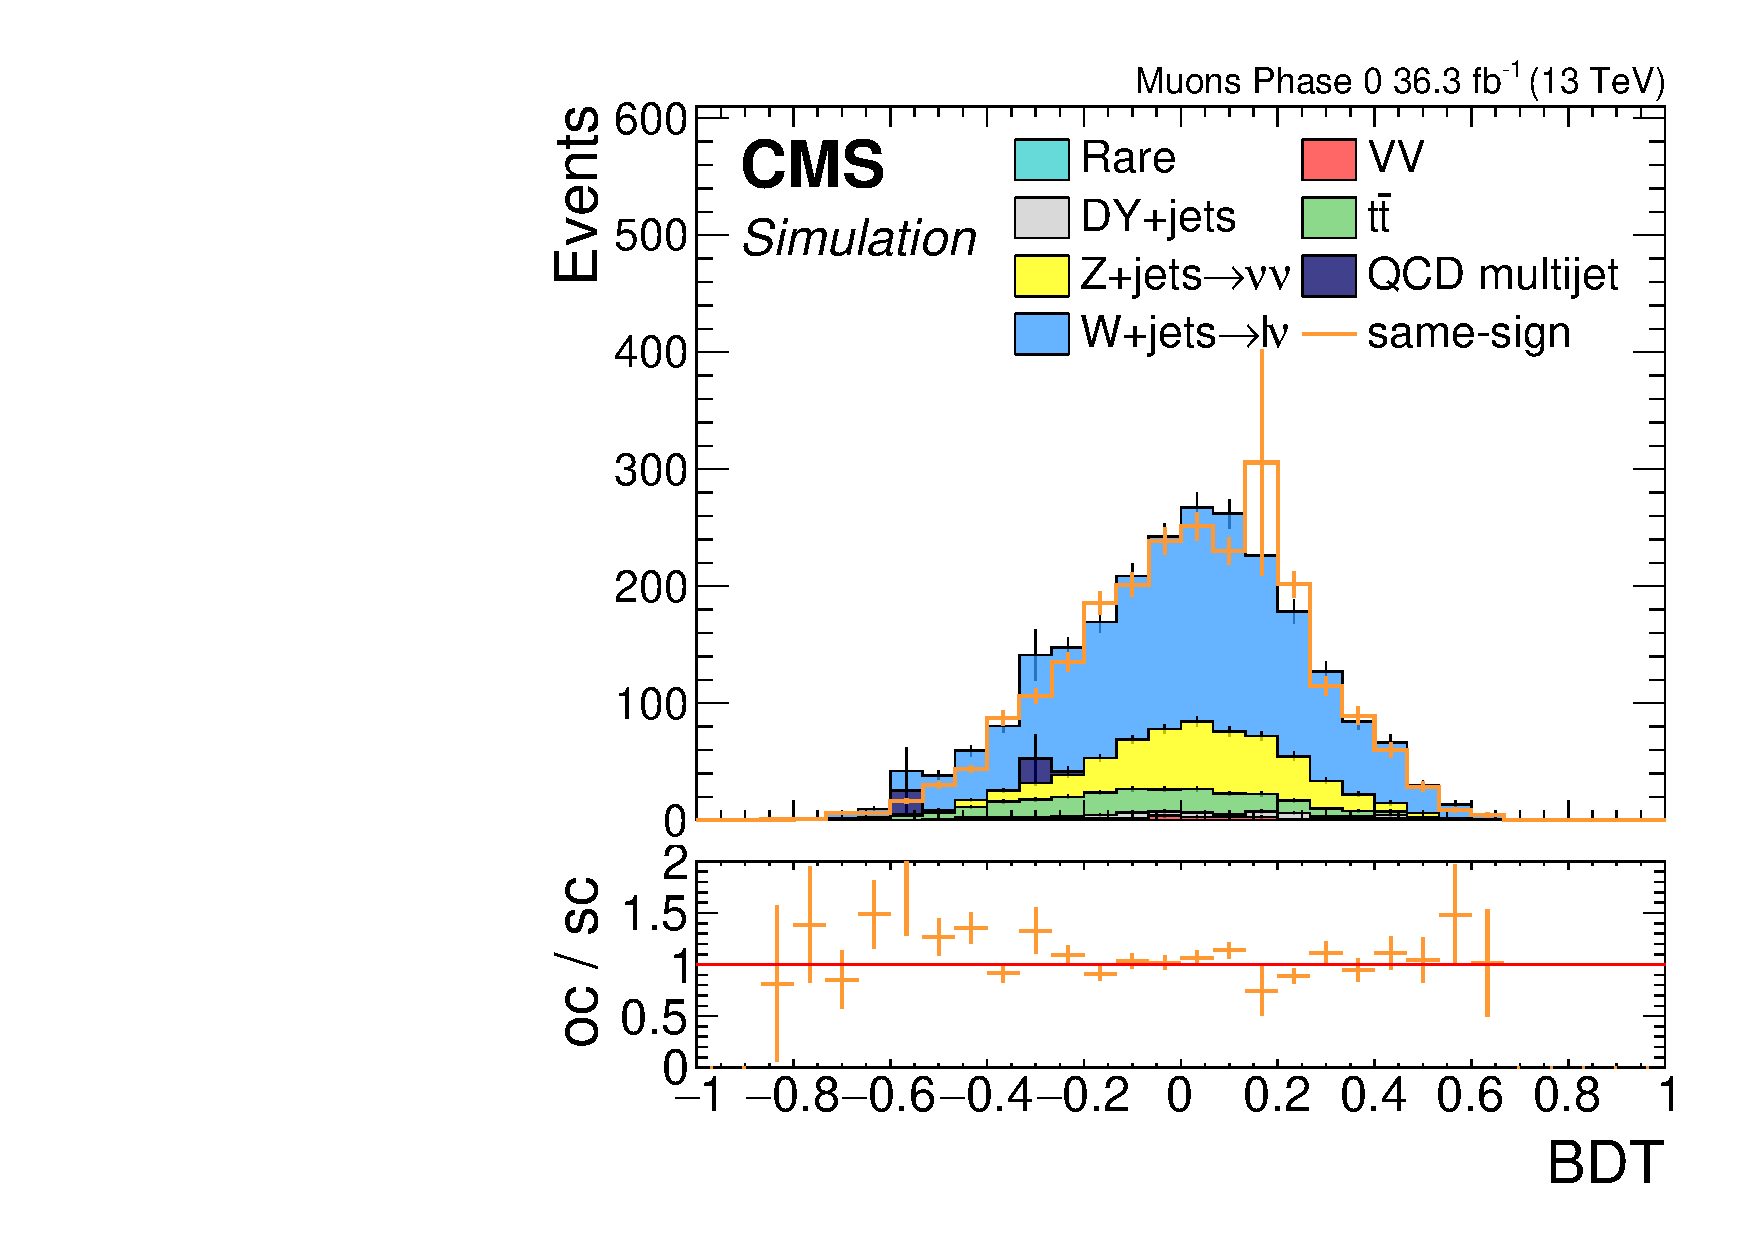
\includegraphics[width=0.48\linewidth]{plots/track_muon_sc_comparison/none_exTrack_dilepBDTCorrJetNoMultIso10Dr0.6.pdf} \,
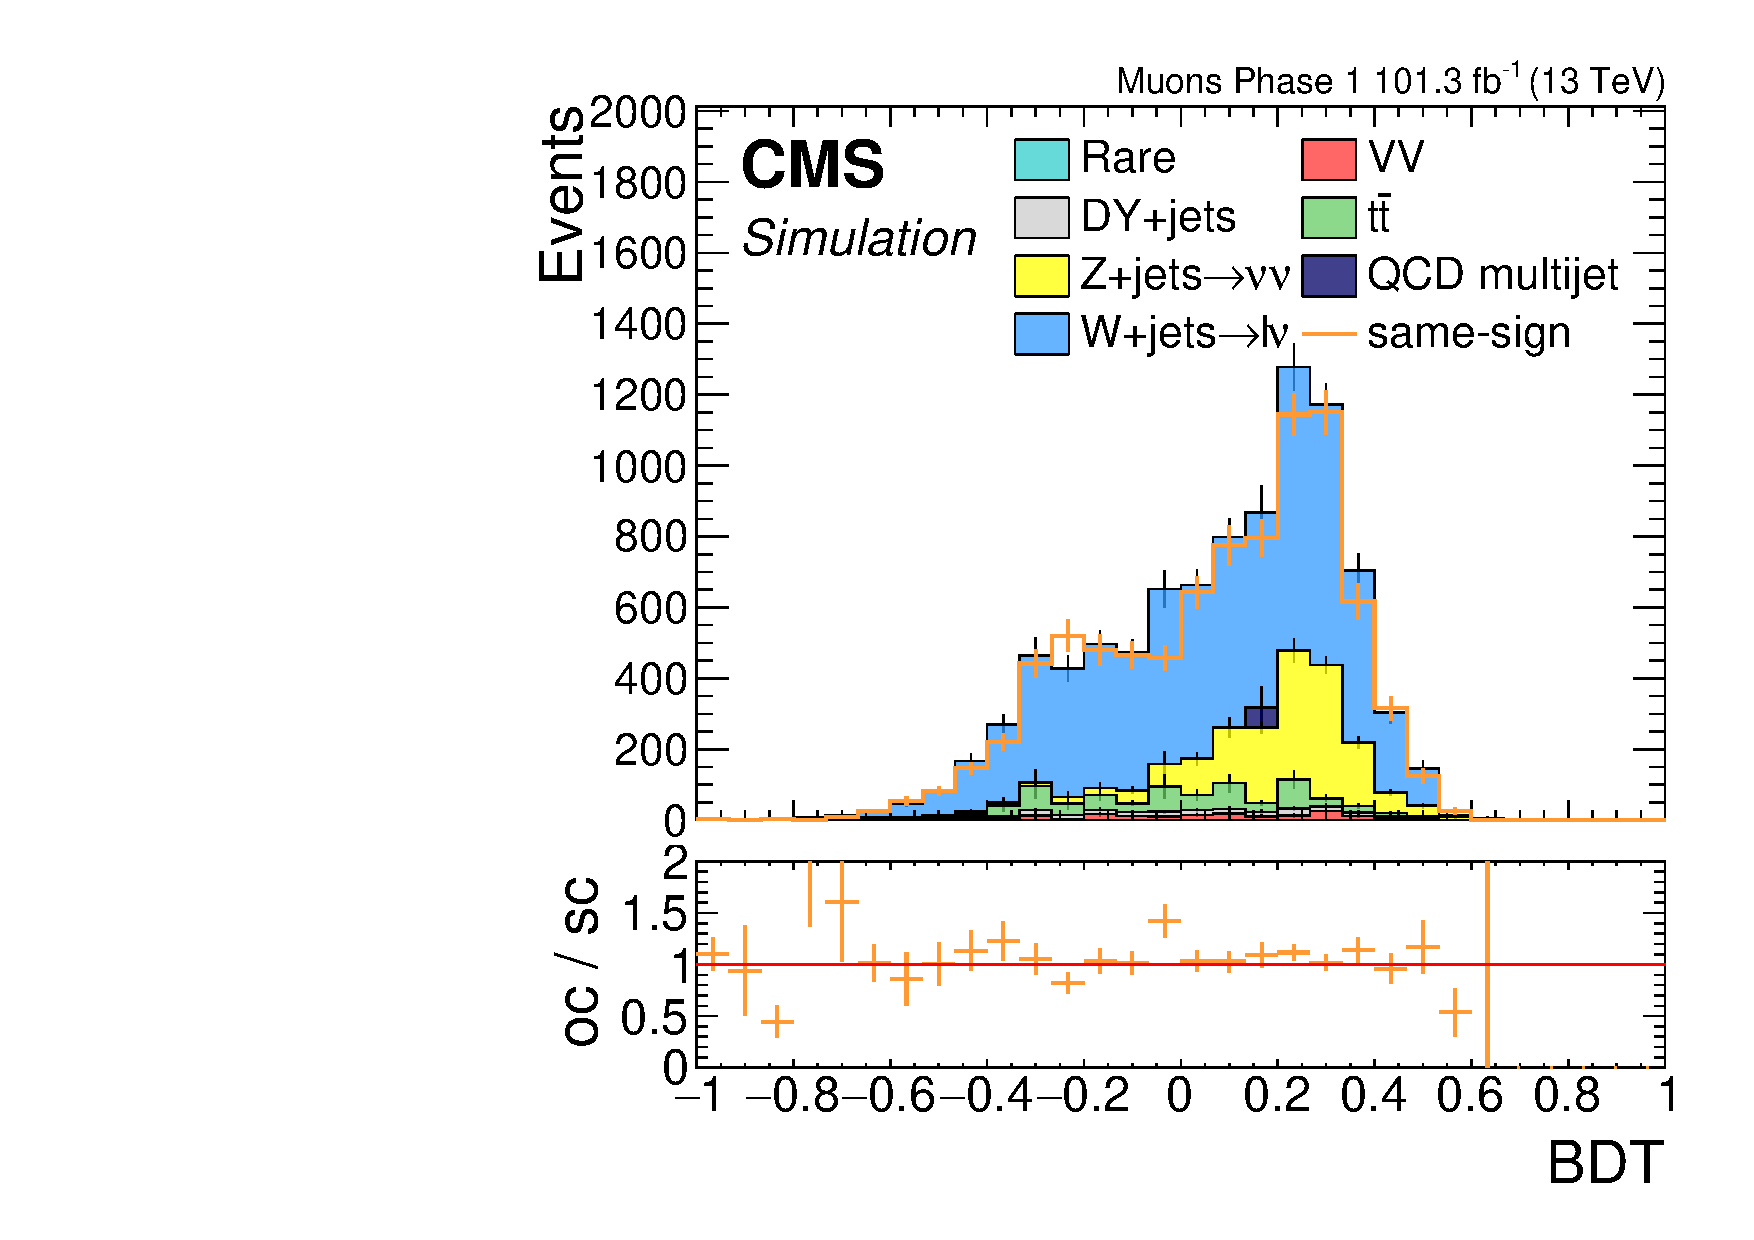
\includegraphics[width=0.48\linewidth]{plots/track_muon_sc_comparison_phase1/none_exTrack_dilepBDTCorrJetNoMultIso10Dr0.6.pdf}  \\
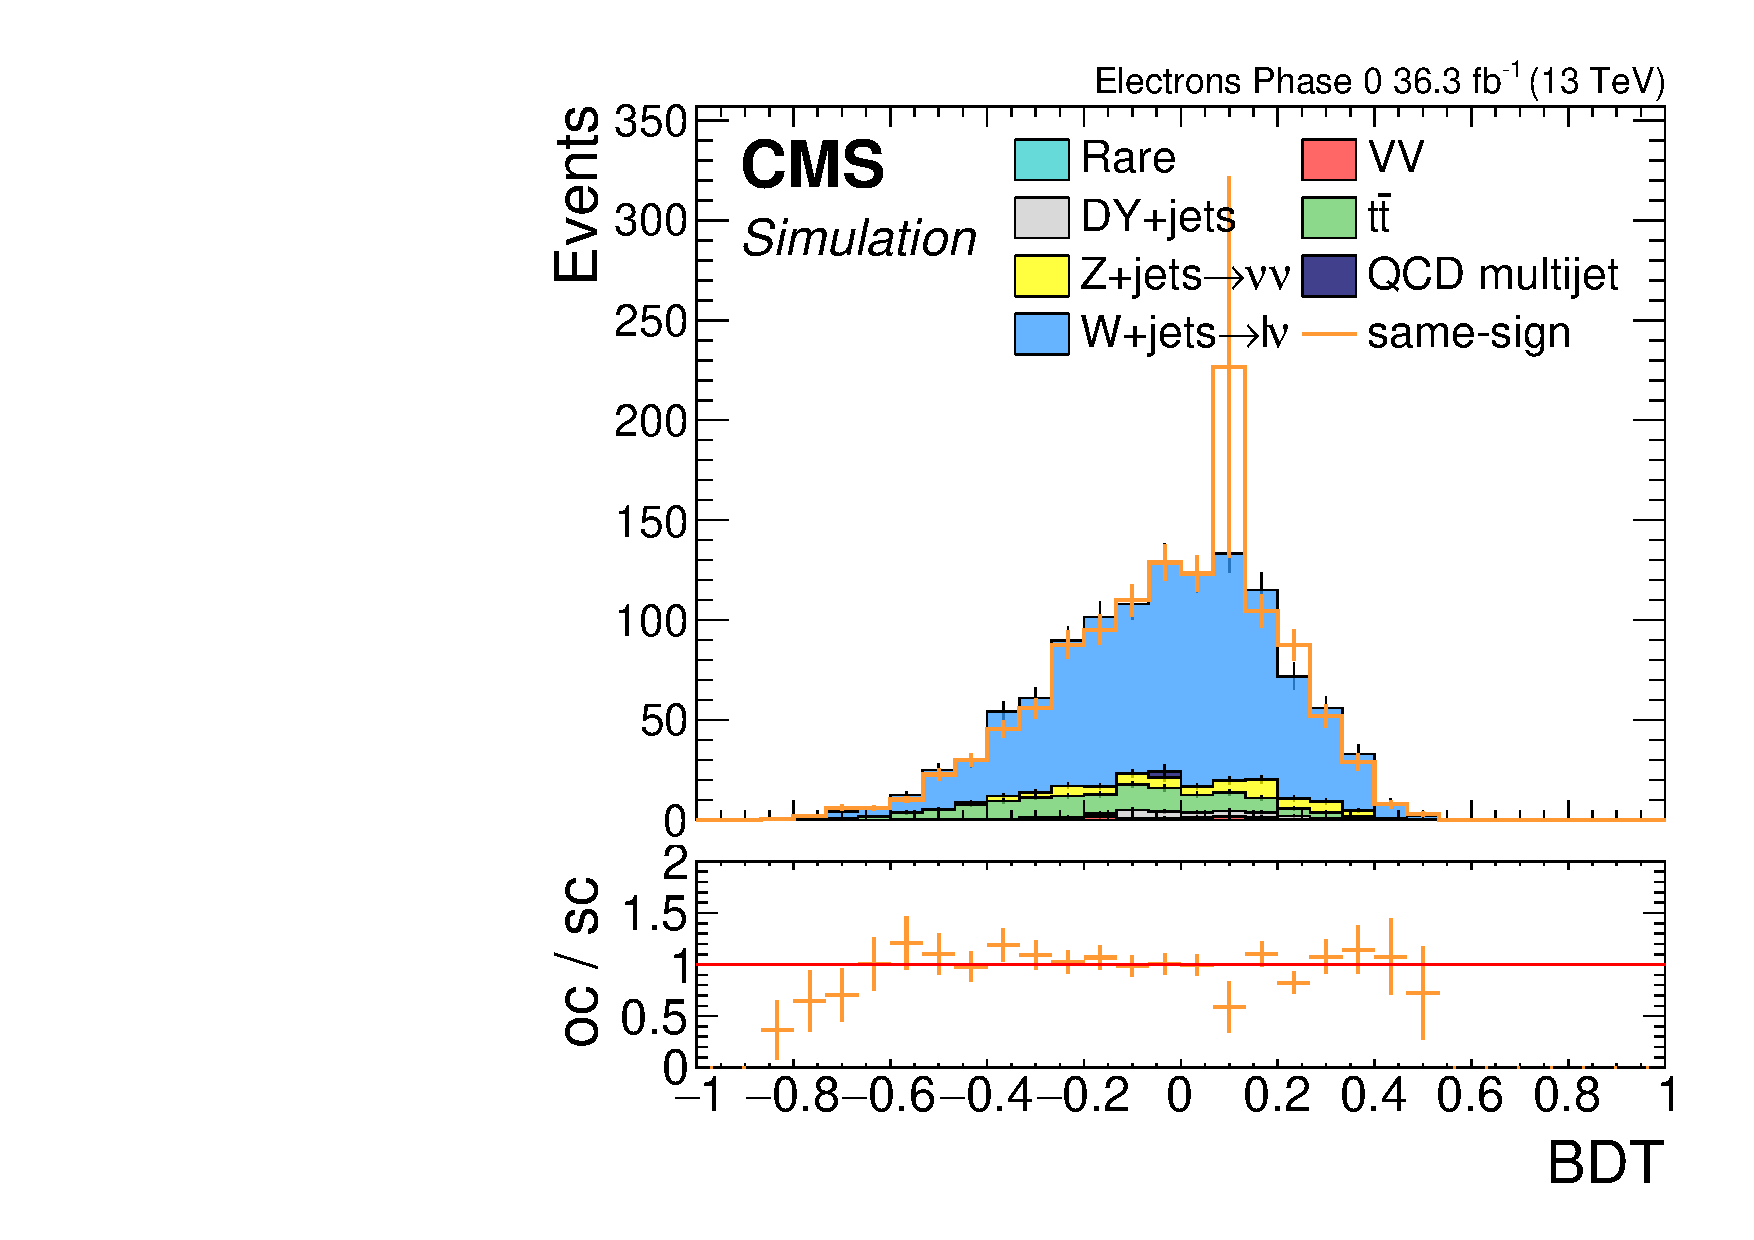
\includegraphics[width=0.48\linewidth]{plots/track_electron_sc_comparison/none_exTrack_dilepBDTCorrJetNoMultIso10Dr0.5.pdf} \,
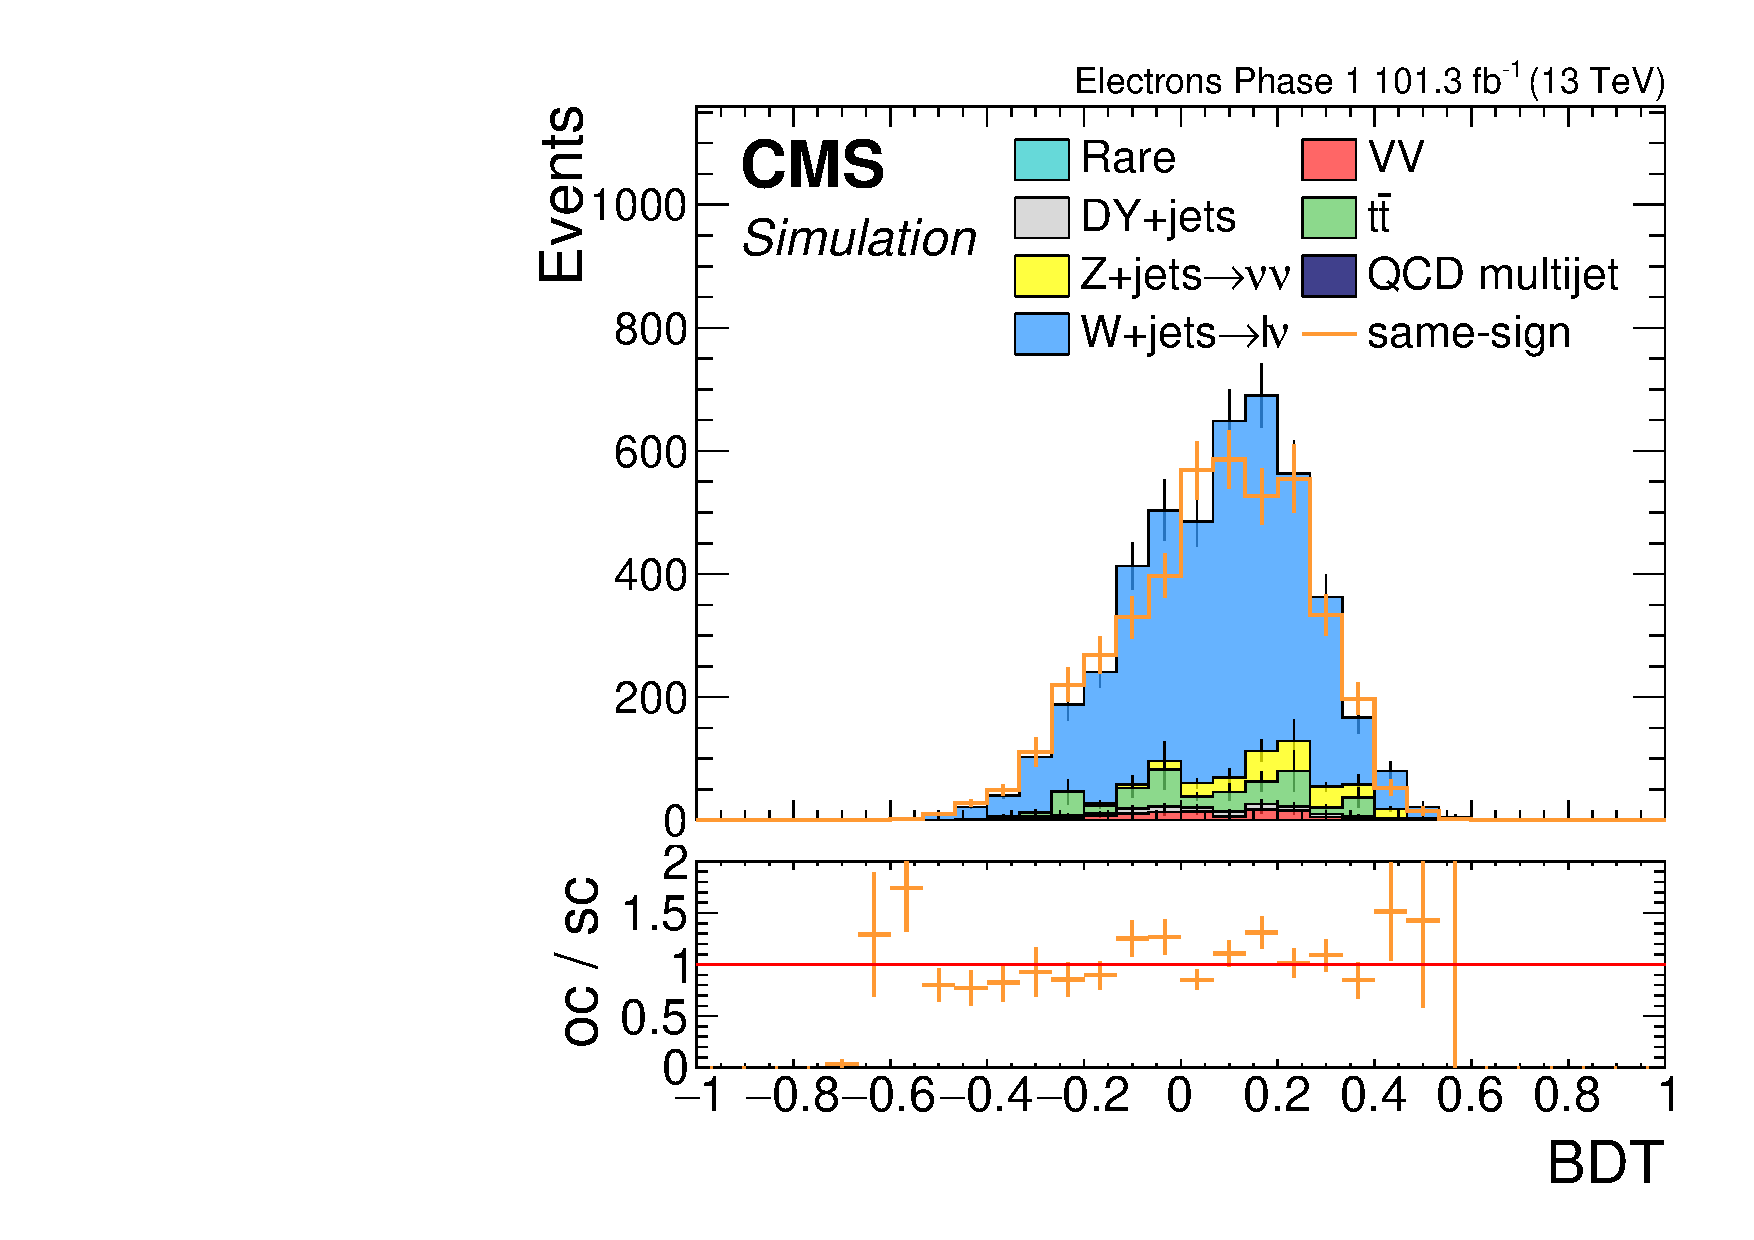
\includegraphics[width=0.48\linewidth]{plots/track_electron_sc_comparison_phase1/none_exTrack_dilepBDTCorrJetNoMultIso10Dr0.5.pdf} \\
\caption[Exclusive track category closure tests]{Distributions constituting the closure tests for the exclusive track background for the muon+track (top) and electron+track (bottom) for Phase 0 (left) and Phase 1 (right). The stacked histograms represent the SM background for OC pairs, while the orange line is the distribution for SC pairs noramlized according to the method. The lower panel shows the ratio between opposite-charge and same-charge counts for each bin. All uncertainties shown are statistical.}
\label{fig:ex-track-closure-tests}
\end{figure}